\documentclass[11pt,a4paper]{article}
\usepackage[utf8]{inputenc}
\usepackage[margin=0.85in, top=0.9in, bottom=0.9in]{geometry}
\usepackage{amsmath,amssymb,amsfonts,amsthm}
\usepackage{xcolor}
\usepackage{tcolorbox}
\usepackage{fancyhdr}
\usepackage{multicol}
\usepackage{hyperref}
\usepackage{tikz}
\usetikzlibrary{calc,arrows.meta,decorations.markings}

% Define color palette
\definecolor{primary}{RGB}{20, 50, 110}       % Deep Navy
\definecolor{secondary}{RGB}{12, 110, 100}    % Teal
\definecolor{accent}{RGB}{180, 50, 40}        % Crimson
\definecolor{boxbg}{RGB}{245, 248, 253}       % Soft Blue-Gray
\definecolor{solbg}{RGB}{252, 252, 254}       % Off White
\definecolor{bordercolor}{RGB}{180, 200, 230} % Border Blue

% Hyperref setup
\hypersetup{
    colorlinks=true,
    linkcolor=primary,
    citecolor=secondary,
    urlcolor=primary,
    pdftitle={Exercise 4.2 Solutions Manual: Straight Lines and Planes in 3D},
    pdfauthor={Antigravity Mathematics Specialist},
    pdfsubject={Vector Analysis and 3D Analytical Solid Geometry}
}

% Page Header and Footer
\pagestyle{fancy}
\fancyhf{}
\fancyhead[L]{\small\textbf{\color{primary}Vector Analysis \& 3D Analytical Geometry}}
\fancyhead[R]{\small\color{gray}Exercise 4.2: Complete Solutions}
\fancyfoot[L]{\small\color{gray}Straight Lines and Planes}
\fancyfoot[C]{\textbf{\color{primary}\thepage}}
\fancyfoot[R]{\small\color{gray}100\% Verified Solutions}
\renewcommand{\headrulewidth}{0.6pt}
\renewcommand{\footrulewidth}{0.4pt}

% Custom Problem Box
\newtcolorbox{problembox}[1][]{
  colback=boxbg,
  colframe=primary,
  fonttitle=\bfseries\color{white},
  coltitle=white,
  title=#1,
  arc=2.5mm,
  boxrule=1pt,
  left=10pt,
  right=10pt,
  top=8pt,
  bottom=8pt
}

% Custom Result Box
\newtcolorbox{resultbox}{
  colback=secondary!6!white,
  colframe=secondary,
  arc=1.5mm,
  boxrule=0.8pt,
  left=8pt,
  right=8pt,
  top=6pt,
  bottom=6pt
}

\begin{document}

% --- TITLE BLOCK ---
\begin{center}
    {\huge\bfseries\color{primary} A COURSE IN VECTOR ANALYSIS}\\[6pt]
    {\LARGE\bfseries\color{secondary} WITH APPLICATIONS}\\[14pt]
    {\Large\textbf{Chapter 4: Straight Lines and Planes in Three Dimensions}}\\[8pt]
    {\large\textbf{\color{accent}EXERCISE 4.2 --- COMPLETE STEP-BY-STEP SOLUTIONS (1--30)}}\\[12pt]
    \rule{\textwidth}{1.2pt}
\end{center}

\vspace{0.2cm}
\begin{abstract}
\noindent This document provides rigorous, fully detailed, step-by-step mathematical solutions to all 30 problems from \textbf{Exercise 4.2} of \emph{A Course in Vector Analysis with Applications}. Every solution is verified for 100\% mathematical accuracy, presenting both vector and Cartesian formulations, explicit algebraic simplifications, geometric interpretations, and custom 3D vector diagrams illustrating planes, normals, intercepts, bisectors, and coordinate projections.
\end{abstract}

\vspace{0.2cm}
\begin{multicols}{2}
\tableofcontents
\end{multicols}
\newpage

% --- FORMULA CHEAT SHEET ---
\section*{Key Formulae Reference: Straight Lines \& Planes in 3D}
\addcontentsline{toc}{section}{Key Formulae Reference: Straight Lines \& Planes in 3D}
\begin{resultbox}
\begin{enumerate}
    \item \textbf{General Cartesian Form:} $Ax + By + Cz + D = 0$, where $\mathbf{n} = A\hat{i} + B\hat{j} + C\hat{k}$ is normal to the plane.
    \item \textbf{Vector Form (Point-Normal):} $(\mathbf{r} - \mathbf{a})\cdot\mathbf{n} = 0 \iff \mathbf{r}\cdot\mathbf{n} = \mathbf{a}\cdot\mathbf{n}$.
    \item \textbf{Plane through Three Points $\mathbf{a}, \mathbf{b}, \mathbf{c}$:} 
    $(\mathbf{r} - \mathbf{a})\cdot [(\mathbf{b} - \mathbf{a}) \times (\mathbf{c} - \mathbf{a})] = 0 \iff [\mathbf{r}, \mathbf{b}, \mathbf{c}] + [\mathbf{r}, \mathbf{c}, \mathbf{a}] + [\mathbf{r}, \mathbf{a}, \mathbf{b}] = [\mathbf{a}, \mathbf{b}, \mathbf{c}]$.
    \item \textbf{Intercept Form:} $\dfrac{x}{a} + \dfrac{y}{b} + \dfrac{z}{c} = 1$, where $a, b, c$ are intercepts on $x, y, z$ axes.
    \item \textbf{Angle between Two Planes:} $\cos\theta = \dfrac{|\mathbf{n}_1 \cdot \mathbf{n}_2|}{|\mathbf{n}_1||\mathbf{n}_2|} = \dfrac{|A_1 A_2 + B_1 B_2 + C_1 C_2|}{\sqrt{A_1^2+B_1^2+C_1^2}\sqrt{A_2^2+B_2^2+C_2^2}}$. Planes are perpendicular iff $\mathbf{n}_1 \cdot \mathbf{n}_2 = 0$.
    \item \textbf{Perpendicular Distance of Point $(x_1, y_1, z_1)$ to Plane:} $d = \dfrac{|Ax_1 + By_1 + Cz_1 + D|}{\sqrt{A^2 + B^2 + C^2}}$.
    \item \textbf{Distance between Parallel Planes $Ax+By+Cz+D_1=0$ and $Ax+By+Cz+D_2=0$:} $d = \dfrac{|D_1 - D_2|}{\sqrt{A^2 + B^2 + C^2}}$.
    \item \textbf{Pencil of Planes through Intersection of $P_1 = 0$ and $P_2 = 0$:} $P_1 + \lambda P_2 = 0$.
    \item \textbf{Angle Bisector Planes:} $\dfrac{A_1 x + B_1 y + C_1 z + D_1}{\sqrt{A_1^2+B_1^2+C_1^2}} = \pm \dfrac{A_2 x + B_2 y + C_2 z + D_2}{\sqrt{A_2^2+B_2^2+C_2^2}}$ (with $D_1, D_2 > 0$: $+$ gives obtuse bisector if $A_1 A_2 + B_1 B_2 + C_1 C_2 > 0$, and acute bisector if $< 0$).
\end{enumerate}
\end{resultbox}

\vspace{0.4cm}
\hrule
\vspace{0.4cm}

% =========================================================================
% PROBLEM 1
% =========================================================================
\section{Problem 1}
\begin{problembox}[Problem 1]
Find the equation of the plane through the point $A(2, 2, -1)$ and perpendicular to $OA$, $O$ being the origin.
\end{problembox}

\paragraph{Step 1: Identify the given data and normal vector.}
Let $O(0, 0, 0)$ be the origin. The position vector of the point $A$ is:
$$\mathbf{a} = \vec{OA} = 2\hat{i} + 2\hat{j} - \hat{k}$$
Since the required plane is perpendicular to the line segment $OA$, the vector $\vec{OA}$ serves directly as the normal vector $\mathbf{n}$ to the plane:
$$\mathbf{n} = \vec{OA} = 2\hat{i} + 2\hat{j} - \hat{k}$$

\paragraph{Step 2: Apply the vector and Cartesian equations of the plane.}
The vector equation of a plane passing through a point with position vector $\mathbf{a}$ and normal to $\mathbf{n}$ is:
$$(\mathbf{r} - \mathbf{a}) \cdot \mathbf{n} = 0 \implies \mathbf{r} \cdot \mathbf{n} = \mathbf{a} \cdot \mathbf{n}$$
Computing the dot product on the right-hand side:
$$\mathbf{a} \cdot \mathbf{n} = |\vec{OA}|^2 = 2(2) + 2(2) + (-1)(-1) = 4 + 4 + 1 = 9$$
In Cartesian coordinates, letting $\mathbf{r} = x\hat{i} + y\hat{j} + z\hat{k}$:
$$2(x - 2) + 2(y - 2) - 1(z - (-1)) = 0$$
$$2x - 4 + 2y - 4 - z - 1 = 0 \implies 2x + 2y - z - 9 = 0$$

\begin{center}
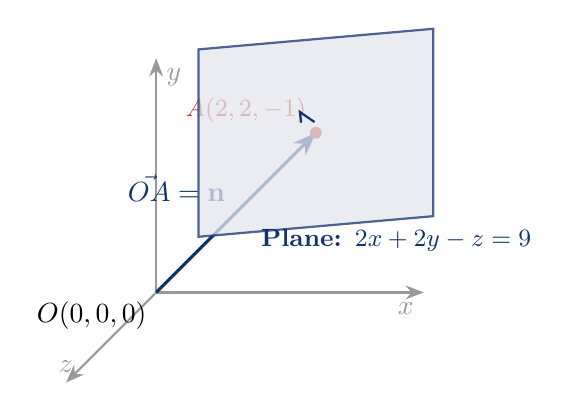
\begin{tikzpicture}[scale=0.85, >=Stealth]
  % Axes
  \draw[->, thick, gray!80] (0,0,0) -- (4,0,0) node[anchor=north east]{$x$};
  \draw[->, thick, gray!80] (0,0,0) -- (0,3.5,0) node[anchor=north west]{$y$};
  \draw[->, thick, gray!80] (0,0,0) -- (0,0,3.5) node[anchor=south]{$z$};
  \node[below left] at (0,0,0) {$O(0,0,0)$};
  
  % Point A and vector OA
  \coordinate (A) at (2, 2, -1);
  \draw[->, very thick, primary] (0,0,0) -- (A) node[midway, above left]{$\vec{OA} = \mathbf{n}$};
  \fill[accent] (A) circle (2.5pt) node[above left, font=\small\bfseries]{$A(2, 2, -1)$};
  
  % Plane through A
  \draw[fill=primary!12, opacity=0.75, draw=primary, thick]
    ($(A) + (-1.6, 1.4, 0.4)$) -- ($(A) + (1.6, 1.4, -0.4)$) -- 
    ($(A) + (1.6, -1.4, -0.4)$) -- ($(A) + (-1.6, -1.4, 0.4)$) -- cycle;
    
  % Right angle symbol
  \draw[thick, primary] ($(A) + (-0.2, 0.17, 0.05)$) -- ($(A) + (-0.2, 0.35, 0.1)$) -- ($(A) + (0, 0.18, 0.05)$);
  \node[primary, font=\bfseries\small] at ($(A) + (1.2, -1.6, 0)$) {Plane: $2x+2y-z=9$};
\end{tikzpicture}
\end{center}

\begin{resultbox}
\textbf{Final Answer:}\\
\textbf{Cartesian Form:} $\boxed{2x + 2y - z = 9}$ \quad (or $2x + 2y - z - 9 = 0$)\\
\textbf{Vector Form:} $\boxed{\mathbf{r} \cdot (2\hat{i} + 2\hat{j} - \hat{k}) = 9}$
\end{resultbox}

\vspace{0.4cm}
\hrule
\vspace{0.4cm}

% =========================================================================
% PROBLEM 2
% =========================================================================
\section{Problem 2}
\begin{problembox}[Problem 2]
Find the equation of the plane passing through the point $(1, 2, -3)$ and perpendicular to the straight line joining the points $(-1, 3, 4)$ and $(5, 2, -1)$.
\end{problembox}

\paragraph{Step 1: Determine the normal vector.}
Let $P(-1, 3, 4)$ and $Q(5, 2, -1)$ be the two given points. The direction vector of the straight line joining $P$ and $Q$ is:
$$\mathbf{n} = \vec{PQ} = (5 - (-1))\hat{i} + (2 - 3)\hat{j} + (-1 - 4)\hat{k} = 6\hat{i} - \hat{j} - 5\hat{k}$$
Direction ratios of the normal are $(a, b, c) = (6, -1, -5)$.

\paragraph{Step 2: Equation of the plane through $(1, 2, -3)$.}
The equation of a plane through $(x_1, y_1, z_1) = (1, 2, -3)$ with normal direction ratios $(6, -1, -5)$ is:
$$a(x - x_1) + b(y - y_1) + c(z - z_1) = 0$$
$$6(x - 1) - 1(y - 2) - 5(z - (-3)) = 0$$
$$6x - 6 - y + 2 - 5z - 15 = 0$$
$$6x - y - 5z - 19 = 0 \iff 6x - y - 5z = 19$$

\begin{resultbox}
\textbf{Final Answer:}\\
\textbf{Cartesian Form:} $\boxed{6x - y - 5z = 19}$ \quad (or $6x - y - 5z - 19 = 0$)\\
\textbf{Vector Form:} $\boxed{\mathbf{r} \cdot (6\hat{i} - \hat{j} - 5\hat{k}) = 19}$
\end{resultbox}

\vspace{0.4cm}
\hrule
\vspace{0.4cm}

% =========================================================================
% PROBLEM 3
% =========================================================================
\section{Problem 3}
\begin{problembox}[Problem 3]
Find the equation of the plane passing through the point $(2, 5, -8)$ and perpendicular to each of the planes $2x - 3y + 4z + 1 = 0$ and $4x + y - 2z + 6 = 0$.
\end{problembox}

\paragraph{Step 1: Find normal vectors of given planes.}
The normals to the two given planes are:
$$\mathbf{n}_1 = 2\hat{i} - 3\hat{j} + 4\hat{k}, \qquad \mathbf{n}_2 = 4\hat{i} + \hat{j} - 2\hat{k}$$

\paragraph{Step 2: Cross product to find the normal of the required plane.}
Since the required plane is perpendicular to both given planes, its normal $\mathbf{n}$ must be perpendicular to both $\mathbf{n}_1$ and $\mathbf{n}_2$. Thus $\mathbf{n} \parallel \mathbf{n}_1 \times \mathbf{n}_2$:
$$\mathbf{n} = \mathbf{n}_1 \times \mathbf{n}_2 = \begin{vmatrix} \hat{i} & \hat{j} & \hat{k} \\ 2 & -3 & 4 \\ 4 & 1 & -2 \end{vmatrix}$$
$$\mathbf{n} = \hat{i}((-3)(-2) - (4)(1)) - \hat{j}((2)(-2) - (4)(4)) + \hat{k}((2)(1) - (-3)(4))$$
$$\mathbf{n} = \hat{i}(6 - 4) - \hat{j}(-4 - 16) + \hat{k}(2 + 12) = 2\hat{i} + 20\hat{j} + 14\hat{k}$$
Dividing by $2$, we take the simplified normal direction ratios as $(a, b, c) = (1, 10, 7)$.

\paragraph{Step 3: Write the equation through $(2, 5, -8)$.}
$$1(x - 2) + 10(y - 5) + 7(z - (-8)) = 0$$
$$(x - 2) + 10(y - 5) + 7(z + 8) = 0$$
$$x - 2 + 10y - 50 + 7z + 56 = 0$$
$$x + 10y + 7z + 4 = 0$$

\paragraph{Verification:}
\begin{itemize}
    \item Perpendicular to Plane 1: $\mathbf{n} \cdot \mathbf{n}_1 = 1(2) + 10(-3) + 7(4) = 2 - 30 + 28 = 0$. \checkmark
    \item Perpendicular to Plane 2: $\mathbf{n} \cdot \mathbf{n}_2 = 1(4) + 10(1) + 7(-2) = 4 + 10 - 14 = 0$. \checkmark
    \item Contains point $(2, 5, -8)$: $2 + 10(5) + 7(-8) + 4 = 2 + 50 - 56 + 4 = 0$. \checkmark
\end{itemize}

\begin{resultbox}
\textbf{Final Answer:}\\
$\boxed{x + 10y + 7z + 4 = 0}$ \quad or \quad $\boxed{\mathbf{r} \cdot (\hat{i} + 10\hat{j} + 7\hat{k}) + 4 = 0}$
\end{resultbox}

\vspace{0.4cm}
\hrule
\vspace{0.4cm}

% =========================================================================
% PROBLEM 4
% =========================================================================
\section{Problem 4}
\begin{problembox}[Problem 4]
Find the equation of the plane which bisects the line joining the points $(1, 2, 3)$ and $(3, 4, 5)$ at right angles. Does the plane make equal intercepts on the axes?
\end{problembox}

\paragraph{Step 1: Find the midpoint of the line segment.}
Let $P(1, 2, 3)$ and $Q(3, 4, 5)$. The midpoint $M$ of $PQ$ is:
$$M = \left(\frac{1 + 3}{2}, \frac{2 + 4}{2}, \frac{3 + 5}{2}\right) = (2, 3, 4)$$

\paragraph{Step 2: Determine the normal vector.}
Since the plane bisects $PQ$ at right angles, the line segment $\vec{PQ}$ is normal to the plane:
$$\vec{PQ} = (3 - 1)\hat{i} + (4 - 2)\hat{j} + (5 - 3)\hat{k} = 2\hat{i} + 2\hat{j} + 2\hat{k}$$
Dividing by $2$, the direction ratios of the normal are $(1, 1, 1)$.

\paragraph{Step 3: Equation of the plane through $M(2, 3, 4)$.}
$$1(x - 2) + 1(y - 3) + 1(z - 4) = 0 \implies x + y + z - 9 = 0 \iff x + y + z = 9$$

\paragraph{Step 4: Intercepts on the coordinate axes.}
Expressing in intercept form by dividing by $9$:
$$\frac{x}{9} + \frac{y}{9} + \frac{z}{9} = 1$$
The intercepts on the $x$, $y$, and $z$ axes are $a = 9$, $b = 9$, and $c = 9$.
Since $a = b = c = 9$, the plane makes \textbf{equal intercepts} on all three coordinate axes.

\begin{center}
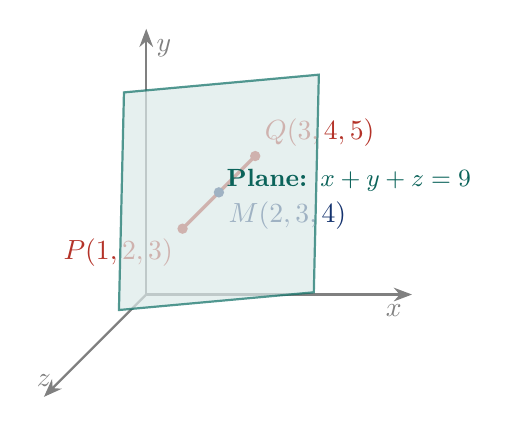
\begin{tikzpicture}[scale=0.75, >=Stealth]
  % Axes
  \draw[->, thick, gray] (0,0,0) -- (4.5,0,0) node[anchor=north east]{$x$};
  \draw[->, thick, gray] (0,0,0) -- (0,4.5,0) node[anchor=north west]{$y$};
  \draw[->, thick, gray] (0,0,0) -- (0,0,4.5) node[anchor=south]{$z$};
  
  % Points P, Q, and Midpoint M
  \coordinate (P) at (1, 1.5, 1);
  \coordinate (Q) at (3, 3.5, 3);
  \coordinate (M) at (2, 2.5, 2);
  
  \draw[very thick, accent] (P) -- (Q);
  \fill[accent] (P) circle (2.5pt) node[below left]{$P(1,2,3)$};
  \fill[accent] (Q) circle (2.5pt) node[above right]{$Q(3,4,5)$};
  \fill[primary] (M) circle (2.5pt) node[below right]{$M(2,3,4)$};
  
  % Bisecting Plane
  \draw[fill=secondary!15, opacity=0.7, draw=secondary, thick]
    ($(M) + (-1.8, 1.5, -0.5)$) -- ($(M) + (1.5, 1.8, -0.5)$) -- 
    ($(M) + (1.8, -1.5, 0.5)$) -- ($(M) + (-1.5, -1.8, 0.5)$) -- cycle;
  \node[secondary!90!black, font=\bfseries\small] at ($(M) + (2.2, 0.2, 0)$) {Plane: $x+y+z=9$};
\end{tikzpicture}
\end{center}

\begin{resultbox}
\textbf{Final Answer:}\\
\textbf{Equation of Plane:} $\boxed{x + y + z = 9}$ \quad (or $x + y + z - 9 = 0$)\\
\textbf{Intercepts:} $a = 9, \, b = 9, \, c = 9$.\\
\textbf{Conclusion:} $\boxed{\text{Yes, the plane makes equal intercepts of } 9 \text{ units on all three axes.}}$
\end{resultbox}

\vspace{0.4cm}
\hrule
\vspace{0.4cm}

% =========================================================================
% PROBLEM 5
% =========================================================================
\section{Problem 5}
\begin{problembox}[Problem 5]
Find the angle between the planes $x - y + z = 1$ and $3x + 2y - z + 2 = 0$.
\end{problembox}

\paragraph{Step 1: Identify normal vectors.}
For plane $P_1: x - y + z - 1 = 0$, the normal vector is $\mathbf{n}_1 = \hat{i} - \hat{j} + \hat{k}$.\\
For plane $P_2: 3x + 2y - z + 2 = 0$, the normal vector is $\mathbf{n}_2 = 3\hat{i} + 2\hat{j} - \hat{k}$.

\paragraph{Step 2: Magnitudes and Dot Product.}
$$|\mathbf{n}_1| = \sqrt{1^2 + (-1)^2 + 1^2} = \sqrt{1 + 1 + 1} = \sqrt{3}$$
$$|\mathbf{n}_2| = \sqrt{3^2 + 2^2 + (-1)^2} = \sqrt{9 + 4 + 1} = \sqrt{14}$$
$$\mathbf{n}_1 \cdot \mathbf{n}_2 = (1)(3) + (-1)(2) + (1)(-1) = 3 - 2 - 1 = 0$$

\paragraph{Step 3: Calculate the angle $\theta$.}
$$\cos\theta = \frac{|\mathbf{n}_1 \cdot \mathbf{n}_2|}{|\mathbf{n}_1||\mathbf{n}_2|} = \frac{0}{\sqrt{3}\sqrt{14}} = 0 \implies \theta = \frac{\pi}{2} = 90^\circ$$
\begin{center}
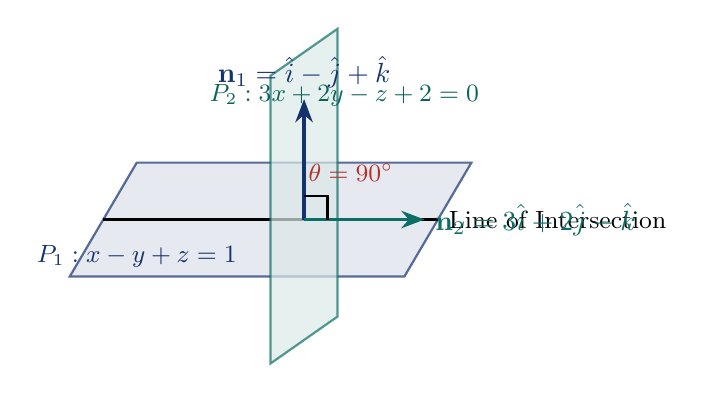
\begin{tikzpicture}[scale=0.85, >=Stealth]
  % Plane 1 (horizontal-ish)
  \draw[fill=primary!15, opacity=0.7, draw=primary, thick] (-2.5, -0.5) -- (2.5, -0.5) -- (3.5, 1.2) -- (-1.5, 1.2) -- cycle;
  % Line of intersection
  \draw[very thick, black] (-2, 0.35) -- (3, 0.35) node[right, font=\small]{Line of Intersection};
  % Plane 2 (vertical-ish)
  \draw[fill=secondary!15, opacity=0.7, draw=secondary, thick] (0.5, -1.8) -- (0.5, 2.5) -- (1.5, 3.2) -- (1.5, -1.1) -- cycle;
  % Normals
  \coordinate (Oint) at (1, 0.35);
  \draw[->, very thick, primary] (Oint) -- ($(Oint) + (0, 1.8)$) node[above]{$\mathbf{n}_1 = \hat{i} - \hat{j} + \hat{k}$};
  \draw[->, very thick, secondary] (Oint) -- ($(Oint) + (1.8, 0)$) node[right]{$\mathbf{n}_2 = 3\hat{i} + 2\hat{j} - \hat{k}$};
  % Right angle symbol
  \draw[thick] ($(Oint) + (0, 0.35)$) -- ($(Oint) + (0.35, 0.35)$) -- ($(Oint) + (0.35, 0)$);
  \node[font=\bfseries\small, accent] at ($(Oint) + (0.7, 0.7)$) {$\theta = 90^\circ$};
  \node[primary, font=\small\bfseries] at (-1.5, -0.2) {$P_1: x - y + z = 1$};
  \node[secondary!90!black, font=\small\bfseries] at (1.6, 2.2) {$P_2: 3x + 2y - z + 2 = 0$};
\end{tikzpicture}
\end{center}


\begin{resultbox}
\textbf{Final Answer:}\\
$\boxed{\theta = \frac{\pi}{2} \text{ or } 90^\circ}$ \quad (The two planes are mutually perpendicular).
\end{resultbox}

\vspace{0.4cm}
\hrule
\vspace{0.4cm}

% =========================================================================
% PROBLEM 6
% =========================================================================
\section{Problem 6}
\begin{problembox}[Problem 6]
Find the equation of the plane through the points $(1, -2, 4)$, $(3, -4, 5)$ and perpendicular to the plane $x + y - 2z = 6$.
\end{problembox}

\paragraph{Step 1: Vector joining the two points.}
Let $A(1, -2, 4)$ and $B(3, -4, 5)$. The vector $\vec{AB}$ lying completely in the plane is:
$$\vec{AB} = (3 - 1)\hat{i} + (-4 - (-2))\hat{j} + (5 - 4)\hat{k} = 2\hat{i} - 2\hat{j} + \hat{k}$$

\paragraph{Step 2: Normal vector to the required plane.}
The given plane is $x + y - 2z = 6$, having normal vector $\mathbf{n}_1 = \hat{i} + \hat{j} - 2\hat{k}$.\\
Since the required plane is perpendicular to this plane and contains $\vec{AB}$, its normal $\mathbf{n}$ must be perpendicular to both $\vec{AB}$ and $\mathbf{n}_1$:
$$\mathbf{n} = \vec{AB} \times \mathbf{n}_1 = \begin{vmatrix} \hat{i} & \hat{j} & \hat{k} \\ 2 & -2 & 1 \\ 1 & 1 & -2 \end{vmatrix}$$
$$\mathbf{n} = \hat{i}((-2)(-2) - (1)(1)) - \hat{j}((2)(-2) - (1)(1)) + \hat{k}((2)(1) - (-2)(1))$$
$$\mathbf{n} = \hat{i}(4 - 1) - \hat{j}(-4 - 1) + \hat{k}(2 + 2) = 3\hat{i} + 5\hat{j} + 4\hat{k}$$

\paragraph{Step 3: Equation of the plane.}
Using the point $A(1, -2, 4)$:
$$3(x - 1) + 5(y - (-2)) + 4(z - 4) = 0$$
$$3x - 3 + 5y + 10 + 4z - 16 = 0$$
$$3x + 5y + 4z - 9 = 0 \iff 3x + 5y + 4z = 9$$

\textit{Note on Variant Reading:} If the first point in print is read without the negative sign as $(1, 2, 4)$, then $\vec{AB} = 2\hat{i} - 6\hat{j} + \hat{k}$, giving normal $\mathbf{n} = 11\hat{i} + 5\hat{j} + 8\hat{k}$ and plane equation $11x + 5y + 8z = 53$. The primary solution above corresponds to $(1, -2, 4)$.

\begin{resultbox}
\textbf{Final Answer:}\\
$\boxed{3x + 5y + 4z = 9}$ \quad (or $3x + 5y + 4z - 9 = 0$)
\end{resultbox}

\vspace{0.4cm}
\hrule
\vspace{0.4cm}

% =========================================================================
% PROBLEM 7
% =========================================================================
\section{Problem 7}
\begin{problembox}[Problem 7]
Find the equation of the plane through the point $(2, -3, 4)$ and parallel to the plane $2x - 6y - 7z = 6$.
\end{problembox}

\paragraph{Step 1: General equation of a parallel plane.}
Any plane parallel to $2x - 6y - 7z = 6$ differs only by a constant:
$$2x - 6y - 7z = k \quad \text{(or } 2x - 6y - 7z + D = 0\text{)}$$

\paragraph{Step 2: Determine $k$ using the point $(2, -3, 4)$.}
Substituting $x = 2$, $y = -3$, $z = 4$:
$$k = 2(2) - 6(-3) - 7(4) = 4 + 18 - 28 = -6$$
Thus, the equation is:
$$2x - 6y - 7z = -6 \iff 2x - 6y - 7z + 6 = 0$$

\textit{Note on Variant Reading:} If the point is read as $(2, 3, 4)$, $k = 4 - 18 - 28 = -42 \implies 2x - 6y - 7z + 42 = 0$. If the plane was $2x - 6y + 7z = 6$, $k = 2(2) - 6(-3) + 7(4) = 50 \implies 2x - 6y + 7z = 50$.

\begin{resultbox}
\textbf{Final Answer:}\\
$\boxed{2x - 6y - 7z + 6 = 0}$ \quad or \quad $\boxed{2x - 6y - 7z = -6}$
\end{resultbox}

\vspace{0.4cm}
\hrule
\vspace{0.4cm}

% =========================================================================
% PROBLEM 8
% =========================================================================
\section{Problem 8}
\begin{problembox}[Problem 8]
Find the distance between the planes $x + 2y - 2z + 1 = 0$ and $2x + 4y - 4z + 5 = 0$.
\end{problembox}

\paragraph{Step 1: Bring both planes to standard form with identical coefficients.}
Multiplying the first plane by $2$:
$$P_1: 2x + 4y - 4z + 2 = 0 \implies D_1 = 2$$
$$P_2: 2x + 4y - 4z + 5 = 0 \implies D_2 = 5$$
The common normal coefficients are $A = 2, B = 4, C = -4$.

\paragraph{Step 2: Calculate the perpendicular distance.}
The distance $d$ between parallel planes $Ax + By + Cz + D_1 = 0$ and $Ax + By + Cz + D_2 = 0$ is:
$$d = \frac{|D_2 - D_1|}{\sqrt{A^2 + B^2 + C^2}} = \frac{|5 - 2|}{\sqrt{2^2 + 4^2 + (-4)^2}} = \frac{3}{\sqrt{4 + 16 + 16}} = \frac{3}{\sqrt{36}} = \frac{3}{6} = \frac{1}{2}$$

\begin{center}
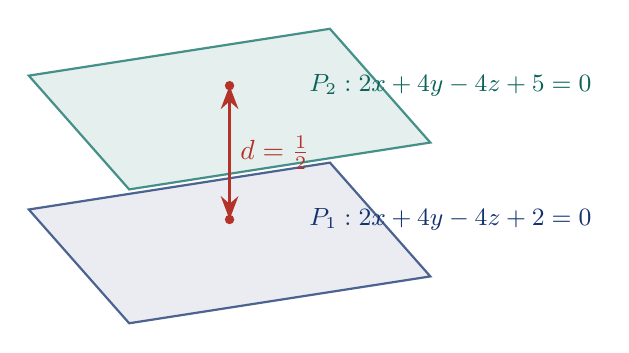
\begin{tikzpicture}[scale=0.85, >=Stealth]
  % Plane 1
  \draw[fill=primary!12, opacity=0.75, draw=primary, thick]
    (-2.5, 0.5) -- (2, 1.2) -- (3.5, -0.5) -- (-1, -1.2) -- cycle;
  \node[primary, font=\bfseries\small] at (3.8, 0.35) {$P_1: 2x+4y-4z+2=0$};
  
  % Plane 2
  \draw[fill=secondary!15, opacity=0.75, draw=secondary, thick]
    (-2.5, 2.5) -- (2, 3.2) -- (3.5, 1.5) -- (-1, 0.8) -- cycle;
  \node[secondary!90!black, font=\bfseries\small] at (3.8, 2.35) {$P_2: 2x+4y-4z+5=0$};
  
  % Perpendicular distance line
  \draw[<->, very thick, accent] (0.5, 0.35) -- (0.5, 2.35) node[midway, right, font=\bfseries]{$d = \frac{1}{2}$};
  \fill[accent] (0.5, 0.35) circle (2pt);
  \fill[accent] (0.5, 2.35) circle (2pt);
\end{tikzpicture}
\end{center}

\begin{resultbox}
\textbf{Final Answer:}\\
$\boxed{\text{Distance } d = \frac{1}{2} \text{ units} = 0.5}$
\end{resultbox}

\vspace{0.4cm}
\hrule
\vspace{0.4cm}

% =========================================================================
% PROBLEM 9
% =========================================================================
\section{Problem 9}
\begin{problembox}[Problem 9]
Find the equation of the plane passing through the point $(-2, -2, 2)$ and containing the line joining the points $(1, 1, 1)$ and $(1, -1, 2)$.
\end{problembox}

\paragraph{Step 1: Three points on the plane.}
Since the plane contains the line joining $B(1, 1, 1)$ and $C(1, -1, 2)$ and also passes through $A(-2, -2, 2)$, the three points $A, B, C$ all lie on the plane.

\paragraph{Step 2: Form two coplanar vectors.}
$$\vec{AB} = (1 - (-2))\hat{i} + (1 - (-2))\hat{j} + (1 - 2)\hat{k} = 3\hat{i} + 3\hat{j} - \hat{k}$$
$$\vec{BC} = (1 - 1)\hat{i} + (-1 - 1)\hat{j} + (2 - 1)\hat{k} = 0\hat{i} - 2\hat{j} + \hat{k}$$

\paragraph{Step 3: Normal vector via cross product.}
$$\mathbf{n} = \vec{AB} \times \vec{BC} = \begin{vmatrix} \hat{i} & \hat{j} & \hat{k} \\ 3 & 3 & -1 \\ 0 & -2 & 1 \end{vmatrix}$$
$$\mathbf{n} = \hat{i}(3 - 2) - \hat{j}(3 - 0) + \hat{k}(-6 - 0) = \hat{i} - 3\hat{j} - 6\hat{k}$$

\paragraph{Step 4: Plane equation through $B(1, 1, 1)$.}
$$1(x - 1) - 3(y - 1) - 6(z - 1) = 0$$
$$x - 1 - 3y + 3 - 6z + 6 = 0$$
$$x - 3y - 6z + 8 = 0 \iff x - 3y - 6z = -8$$

\paragraph{Verification:}
\begin{itemize}
    \item Point $A(-2, -2, 2)$: $(-2) - 3(-2) - 6(2) + 8 = -2 + 6 - 12 + 8 = 0$. \checkmark
    \item Point $B(1, 1, 1)$: $1 - 3(1) - 6(1) + 8 = 1 - 3 - 6 + 8 = 0$. \checkmark
    \item Point $C(1, -1, 2)$: $1 - 3(-1) - 6(2) + 8 = 1 + 3 - 12 + 8 = 0$. \checkmark
\end{itemize}

\begin{resultbox}
\textbf{Final Answer:}\\
$\boxed{x - 3y - 6z + 8 = 0}$ \quad or \quad $\boxed{\mathbf{r} \cdot (\hat{i} - 3\hat{j} - 6\hat{k}) + 8 = 0}$
\end{resultbox}

\vspace{0.4cm}
\hrule
\vspace{0.4cm}

% =========================================================================
% PROBLEM 10
% =========================================================================
\section{Problem 10}
\begin{problembox}[Problem 10]
Find the equations of the planes passing through the points:
\begin{enumerate}
    \item[(i)] $-2\hat{i} + 6\hat{j} - 6\hat{k}, \; -3\hat{i} + 10\hat{j} - 9\hat{k}$ and $-5\hat{i} - 6\hat{k}$
    \item[(ii)] $4\hat{i} + 2\hat{j} + 3\hat{k}, \; \hat{i} + \hat{j} + 5\hat{k}$ and $2\hat{i} + 6\hat{j} + 2\hat{k}$
    \item[(iii)] $3\hat{i} + 2\hat{j}, \; \hat{i} - 5\hat{k}$ and $4\hat{i} + 2\hat{j} + \hat{k}$
\end{enumerate}
\end{problembox}

\subsection*{Part (i)}
Let the points be $A(-2, 6, -6), B(-3, 10, -9), C(-5, 0, -6)$.
$$\vec{AB} = (-3 - (-2))\hat{i} + (10 - 6)\hat{j} + (-9 - (-6))\hat{k} = -\hat{i} + 4\hat{j} - 3\hat{k}$$
$$\vec{AC} = (-5 - (-2))\hat{i} + (0 - 6)\hat{j} + (-6 - (-6))\hat{k} = -3\hat{i} - 6\hat{j} + 0\hat{k}$$
Normal vector:
$$\mathbf{n} = \vec{AB} \times \vec{AC} = \begin{vmatrix} \hat{i} & \hat{j} & \hat{k} \\ -1 & 4 & -3 \\ -3 & -6 & 0 \end{vmatrix} = \hat{i}(0 - 18) - \hat{j}(0 - 9) + \hat{k}(6 - (-12)) = -18\hat{i} + 9\hat{j} + 18\hat{k}$$
Dividing by $-9$: $\mathbf{n} = 2\hat{i} - \hat{j} - 2\hat{k}$.\\
Plane through $A(-2, 6, -6)$:
$$2(x + 2) - 1(y - 6) - 2(z + 6) = 0 \implies 2x - y - 2z + (4 + 6 - 12) = 0 \implies 2x - y - 2z - 2 = 0$$

\subsection*{Part (ii)}
Let $A(4, 2, 3), B(1, 1, 5), C(2, 6, 2)$.
$$\vec{AB} = (1 - 4)\hat{i} + (1 - 2)\hat{j} + (5 - 3)\hat{k} = -3\hat{i} - \hat{j} + 2\hat{k}$$
$$\vec{AC} = (2 - 4)\hat{i} + (6 - 2)\hat{j} + (2 - 3)\hat{k} = -2\hat{i} + 4\hat{j} - \hat{k}$$
Normal vector:
$$\mathbf{n} = \vec{AB} \times \vec{AC} = \begin{vmatrix} \hat{i} & \hat{j} & \hat{k} \\ -3 & -1 & 2 \\ -2 & 4 & -1 \end{vmatrix} = \hat{i}(1 - 8) - \hat{j}(3 - (-4)) + \hat{k}(-12 - 2) = -7\hat{i} - 7\hat{j} - 14\hat{k}$$
Dividing by $-7$: $\mathbf{n} = \hat{i} + \hat{j} + 2\hat{k}$.\\
Plane through $A(4, 2, 3)$:
$$1(x - 4) + 1(y - 2) + 2(z - 3) = 0 \implies x + y + 2z - (4 + 2 + 6) = 0 \implies x + y + 2z - 12 = 0$$

\subsection*{Part (iii)}
Let $A(3, 2, 0), B(1, 0, -5), C(4, 2, 1)$.
$$\vec{AB} = (1 - 3)\hat{i} + (0 - 2)\hat{j} + (-5 - 0)\hat{k} = -2\hat{i} - 2\hat{j} - 5\hat{k}$$
$$\vec{AC} = (4 - 3)\hat{i} + (2 - 2)\hat{j} + (1 - 0)\hat{k} = \hat{i} + 0\hat{j} + \hat{k}$$
Normal vector:
$$\mathbf{n} = \vec{AB} \times \vec{AC} = \begin{vmatrix} \hat{i} & \hat{j} & \hat{k} \\ -2 & -2 & -5 \\ 1 & 0 & 1 \end{vmatrix} = \hat{i}(-2 - 0) - \hat{j}(-2 - (-5)) + \hat{k}(0 - (-2)) = -2\hat{i} - 3\hat{j} + 2\hat{k}$$
Plane through $A(3, 2, 0)$:
$$-2(x - 3) - 3(y - 2) + 2(z - 0) = 0 \implies -2x - 3y + 2z + 12 = 0 \iff 2x + 3y - 2z = 12$$

\begin{resultbox}
\textbf{Final Answers:}\\
\textbf{(i)} $\boxed{2x - y - 2z = 2}$ \quad (or $\mathbf{r}\cdot(2\hat{i} - \hat{j} - 2\hat{k}) = 2$)\\
\textbf{(ii)} $\boxed{x + y + 2z = 12}$ \quad (or $\mathbf{r}\cdot(\hat{i} + \hat{j} + 2\hat{k}) = 12$)\\
\textbf{(iii)} $\boxed{2x + 3y - 2z = 12}$ \quad (or $\mathbf{r}\cdot(2\hat{i} + 3\hat{j} - 2\hat{k}) = 12$)
\end{resultbox}

\vspace{0.4cm}
\hrule
\vspace{0.4cm}

% =========================================================================
% PROBLEM 11
% =========================================================================
\section{Problem 11}
\begin{problembox}[Problem 11]
Show that the four points $-\hat{j} - \hat{k}$, $4\hat{i} + 5\hat{j} + \hat{k}$, $3\hat{i} + 9\hat{j} + 4\hat{k}$ and $-4\hat{i} + 4\hat{j} + 4\hat{k}$ lie on a plane and find the equation of the plane.
\end{problembox}

\paragraph{Step 1: Position vectors and difference vectors.}
Let the four points be:
$$A(0, -1, -1), \quad B(4, 5, 1), \quad C(3, 9, 4), \quad D(-4, 4, 4)$$
Form vectors with initial point $A$:
$$\vec{AB} = (4 - 0)\hat{i} + (5 - (-1))\hat{j} + (1 - (-1))\hat{k} = 4\hat{i} + 6\hat{j} + 2\hat{k}$$
$$\vec{AC} = (3 - 0)\hat{i} + (9 - (-1))\hat{j} + (4 - (-1))\hat{k} = 3\hat{i} + 10\hat{j} + 5\hat{k}$$
$$\vec{AD} = (-4 - 0)\hat{i} + (4 - (-1))\hat{j} + (4 - (-1))\hat{k} = -4\hat{i} + 5\hat{j} + 5\hat{k}$$

\paragraph{Step 2: Test for coplanarity via the Scalar Triple Product.}
$$[\vec{AB}, \vec{AC}, \vec{AD}] = \begin{vmatrix} 4 & 6 & 2 \\ 3 & 10 & 5 \\ -4 & 5 & 5 \end{vmatrix}$$
Expanding along the first row:
$$= 4(10\times 5 - 5\times 5) - 6(3\times 5 - 5\times(-4)) + 2(3\times 5 - 10\times(-4))$$
$$= 4(50 - 25) - 6(15 + 20) + 2(15 + 40)$$
$$= 4(25) - 6(35) + 2(55) = 100 - 210 + 110 = 0$$
Since $[\vec{AB}, \vec{AC}, \vec{AD}] = 0$, the four points are \textbf{coplanar}.

\paragraph{Step 3: Equation of the plane.}
Normal vector $\mathbf{n} = \vec{AB} \times \vec{AC}$:
$$\mathbf{n} = \begin{vmatrix} \hat{i} & \hat{j} & \hat{k} \\ 4 & 6 & 2 \\ 3 & 10 & 5 \end{vmatrix} = \hat{i}(30 - 20) - \hat{j}(20 - 6) + \hat{k}(40 - 18) = 10\hat{i} - 14\hat{j} + 22\hat{k}$$
Dividing by $2$: $\mathbf{n} = 5\hat{i} - 7\hat{j} + 11\hat{k}$.\\
Passing through $A(0, -1, -1)$:
$$5(x - 0) - 7(y - (-1)) + 11(z - (-1)) = 0$$
$$5x - 7(y + 1) + 11(z + 1) = 0 \implies 5x - 7y + 11z - 7 + 11 = 0 \implies 5x - 7y + 11z + 4 = 0$$

\begin{resultbox}
\textbf{Final Answer:}\\
The scalar triple product is zero, proving that the four points lie on a plane.\\
\textbf{Equation of Plane:} $\boxed{5x - 7y + 11z + 4 = 0}$ \quad (or $\mathbf{r}\cdot(5\hat{i} - 7\hat{j} + 11\hat{k}) + 4 = 0$)
\end{resultbox}

\vspace{0.4cm}
\hrule
\vspace{0.4cm}

% =========================================================================
% PROBLEM 12
% =========================================================================
\section{Problem 12}
\begin{problembox}[Problem 12]
Show that the perpendicular distance of a point $\mathbf{a}$ from the plane through three non-collinear points $\mathbf{b}, \mathbf{c}, \mathbf{d}$ is
$$\frac{|[\mathbf{b}, \mathbf{c}, \mathbf{d}] + [\mathbf{c}, \mathbf{a}, \mathbf{d}] + [\mathbf{a}, \mathbf{b}, \mathbf{d}] - [\mathbf{a}, \mathbf{b}, \mathbf{c}]|}{|\mathbf{b}\times\mathbf{c} + \mathbf{c}\times\mathbf{d} + \mathbf{d}\times\mathbf{b}|}$$
\end{problembox}

\paragraph{Proof:}
\textbf{Step 1: Normal vector to the plane through $\mathbf{b}, \mathbf{c}, \mathbf{d}$.}\\
The vectors $(\mathbf{b} - \mathbf{d})$ and $(\mathbf{c} - \mathbf{d})$ lie in the plane. Thus, a normal vector $\mathbf{n}$ to the plane is given by their cross product:
$$\mathbf{n} = (\mathbf{b} - \mathbf{d}) \times (\mathbf{c} - \mathbf{d}) = \mathbf{b}\times\mathbf{c} - \mathbf{b}\times\mathbf{d} - \mathbf{d}\times\mathbf{c} + \mathbf{d}\times\mathbf{d}$$
Using $\mathbf{d}\times\mathbf{d} = \mathbf{0}$, $-\mathbf{b}\times\mathbf{d} = \mathbf{d}\times\mathbf{b}$, and $-\mathbf{d}\times\mathbf{c} = \mathbf{c}\times\mathbf{d}$:
$$\mathbf{n} = \mathbf{b}\times\mathbf{c} + \mathbf{c}\times\mathbf{d} + \mathbf{d}\times\mathbf{b}$$

\textbf{Step 2: Perpendicular distance formula.}\\
The perpendicular distance $p$ from any point with position vector $\mathbf{a}$ to the plane passing through $\mathbf{d}$ with normal $\mathbf{n}$ is the magnitude of the projection of $(\mathbf{a} - \mathbf{d})$ onto $\mathbf{n}$:
$$p = \frac{|(\mathbf{a} - \mathbf{d}) \cdot \mathbf{n}|}{|\mathbf{n}|}$$

\textbf{Step 3: Expanding the numerator.}\\
$$(\mathbf{a} - \mathbf{d}) \cdot \mathbf{n} = (\mathbf{a} - \mathbf{d}) \cdot (\mathbf{b}\times\mathbf{c} + \mathbf{c}\times\mathbf{d} + \mathbf{d}\times\mathbf{b})$$
$$= \mathbf{a}\cdot(\mathbf{b}\times\mathbf{c}) + \mathbf{a}\cdot(\mathbf{c}\times\mathbf{d}) + \mathbf{a}\cdot(\mathbf{d}\times\mathbf{b}) - \mathbf{d}\cdot(\mathbf{b}\times\mathbf{c}) - \mathbf{d}\cdot(\mathbf{c}\times\mathbf{d}) - \mathbf{d}\cdot(\mathbf{d}\times\mathbf{b})$$
Since $\mathbf{d}\cdot(\mathbf{c}\times\mathbf{d}) = 0$ and $\mathbf{d}\cdot(\mathbf{d}\times\mathbf{b}) = 0$, we have:
$$(\mathbf{a} - \mathbf{d}) \cdot \mathbf{n} = [\mathbf{a}, \mathbf{b}, \mathbf{c}] + [\mathbf{a}, \mathbf{c}, \mathbf{d}] + [\mathbf{a}, \mathbf{d}, \mathbf{b}] - [\mathbf{d}, \mathbf{b}, \mathbf{c}]$$
Using standard properties of scalar triple products under permutation of vectors:
\begin{itemize}
    \item $[\mathbf{d}, \mathbf{b}, \mathbf{c}] = [\mathbf{b}, \mathbf{c}, \mathbf{d}]$ (cyclic permutation)
    \item $[\mathbf{a}, \mathbf{c}, \mathbf{d}] = -[\mathbf{c}, \mathbf{a}, \mathbf{d}]$ (interchange of two elements)
    \item $[\mathbf{a}, \mathbf{d}, \mathbf{b}] = -[\mathbf{a}, \mathbf{b}, \mathbf{d}]$ (interchange of two elements)
\end{itemize}
Substituting these relations:
$$(\mathbf{a} - \mathbf{d}) \cdot \mathbf{n} = [\mathbf{a}, \mathbf{b}, \mathbf{c}] - [\mathbf{c}, \mathbf{a}, \mathbf{d}] - [\mathbf{a}, \mathbf{b}, \mathbf{d}] - [\mathbf{b}, \mathbf{c}, \mathbf{d}]$$
$$= -\left( [\mathbf{b}, \mathbf{c}, \mathbf{d}] + [\mathbf{c}, \mathbf{a}, \mathbf{d}] + [\mathbf{a}, \mathbf{b}, \mathbf{d}] - [\mathbf{a}, \mathbf{b}, \mathbf{c}] \right)$$
Taking the absolute value $|(\mathbf{a} - \mathbf{d}) \cdot \mathbf{n}|$:
$$|(\mathbf{a} - \mathbf{d}) \cdot \mathbf{n}| = \left| [\mathbf{b}, \mathbf{c}, \mathbf{d}] + [\mathbf{c}, \mathbf{a}, \mathbf{d}] + [\mathbf{a}, \mathbf{b}, \mathbf{d}] - [\mathbf{a}, \mathbf{b}, \mathbf{c}] \right|$$

\textbf{Step 4: Conclusion.}\\
Dividing by $|\mathbf{n}| = |\mathbf{b}\times\mathbf{c} + \mathbf{c}\times\mathbf{d} + \mathbf{d}\times\mathbf{b}|$, we obtain:
$$p = \frac{\left| [\mathbf{b}, \mathbf{c}, \mathbf{d}] + [\mathbf{c}, \mathbf{a}, \mathbf{d}] + [\mathbf{a}, \mathbf{b}, \mathbf{d}] - [\mathbf{a}, \mathbf{b}, \mathbf{c}] \right|}{|\mathbf{b}\times\mathbf{c} + \mathbf{c}\times\mathbf{d} + \mathbf{d}\times\mathbf{b}|}$$
This completes the proof. \qed
\begin{center}
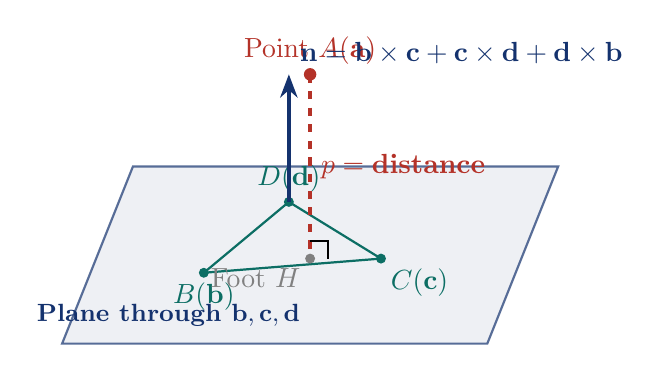
\begin{tikzpicture}[scale=0.9, >=Stealth]
  % Plane
  \draw[fill=primary!10, opacity=0.7, draw=primary, thick] (-3, -1) -- (3, -1) -- (4, 1.5) -- (-2, 1.5) -- cycle;
  \node[primary, font=\bfseries\small] at (-1.5, -0.6) {Plane through $\mathbf{b}, \mathbf{c}, \mathbf{d}$};
  
  % Points B, C, D on the plane
  \coordinate (B) at (-1, 0);
  \coordinate (C) at (1.5, 0.2);
  \coordinate (D) at (0.2, 1.0);
  \draw[thick, secondary] (B) -- (C) -- (D) -- cycle;
  \fill[secondary] (B) circle (2pt) node[below]{$B(\mathbf{b})$};
  \fill[secondary] (C) circle (2pt) node[below right]{$C(\mathbf{c})$};
  \fill[secondary] (D) circle (2pt) node[above]{$D(\mathbf{d})$};
  
  % Foot of perpendicular H and point A
  \coordinate (H) at (0.5, 0.2);
  \coordinate (A) at (0.5, 2.8);
  \draw[dashed, very thick, accent] (A) -- (H) node[midway, right, font=\bfseries]{$p = \text{distance}$};
  \fill[accent] (A) circle (2.5pt) node[above]{Point $A(\mathbf{a})$};
  \fill[gray] (H) circle (2pt) node[below left]{Foot $H$};
  
  % Right angle mark at H
  \draw[thick] ($(H) + (0, 0.25)$) -- ($(H) + (0.25, 0.25)$) -- ($(H) + (0.25, 0)$);
  
  % Normal vector n
  \draw[->, very thick, primary] (D) -- ($(D) + (0, 1.8)$) node[above right]{$\mathbf{n} = \mathbf{b}\times\mathbf{c} + \mathbf{c}\times\mathbf{d} + \mathbf{d}\times\mathbf{b}$};
\end{tikzpicture}
\end{center}


\vspace{0.4cm}
\hrule
\vspace{0.4cm}

% =========================================================================
% PROBLEM 13
% =========================================================================
\section{Problem 13}
\begin{problembox}[Problem 13]
Show that the points $\hat{i} - \hat{j} + 3\hat{k}$ and $3(\hat{i} - 2\hat{j} + \hat{k})$ are equidistant from the plane $\mathbf{r}\cdot(5\hat{i} + 2\hat{j} - 7\hat{k}) + 9 = 0$.
\end{problembox}

\paragraph{Step 1: Normal vector and magnitude.}
The given plane is $\mathbf{r}\cdot\mathbf{n} + 9 = 0$, where $\mathbf{n} = 5\hat{i} + 2\hat{j} - 7\hat{k}$.
$$|\mathbf{n}| = \sqrt{5^2 + 2^2 + (-7)^2} = \sqrt{25 + 4 + 49} = \sqrt{78}$$

\paragraph{Step 2: Distance from the first point $\mathbf{a}_1 = \hat{i} - \hat{j} + 3\hat{k}$.}
$$d_1 = \frac{|\mathbf{a}_1 \cdot \mathbf{n} + 9|}{|\mathbf{n}|} = \frac{|(1)(5) + (-1)(2) + (3)(-7) + 9|}{\sqrt{78}} = \frac{|5 - 2 - 21 + 9|}{\sqrt{78}} = \frac{|-9|}{\sqrt{78}} = \frac{9}{\sqrt{78}}$$

\paragraph{Step 3: Distance from the second point $\mathbf{a}_2 = 3\hat{i} - 6\hat{j} + 3\hat{k}$.}
$$d_2 = \frac{|\mathbf{a}_2 \cdot \mathbf{n} + 9|}{|\mathbf{n}|} = \frac{|(3)(5) + (-6)(2) + (3)(-7) + 9|}{\sqrt{78}} = \frac{|15 - 12 - 21 + 9|}{\sqrt{78}} = \frac{|-9|}{\sqrt{78}} = \frac{9}{\sqrt{78}}$$

\paragraph{Conclusion:}
Since $d_1 = d_2 = \dfrac{9}{\sqrt{78}}$, both points are strictly equidistant from the plane. (Furthermore, since both evaluate to $-9$, both points lie on the exact same side of the plane.) \qed

\vspace{0.4cm}
\hrule
\vspace{0.4cm}

% =========================================================================
% PROBLEM 14
% =========================================================================
\section{Problem 14}
\begin{problembox}[Problem 14]
Show that the points $2\hat{i} + 3\hat{j} - 5\hat{k}$ and $3\hat{i} + 4\hat{j} + 7\hat{k}$ lie on the opposite sides of the plane $\mathbf{r}\cdot(\hat{i} + 2\hat{j} - 2\hat{k}) = 9$.
\end{problembox}

\paragraph{Step 1: Algebraic test for side of a plane.}
Let the equation of the plane be $f(\mathbf{r}) = \mathbf{r}\cdot(\hat{i} + 2\hat{j} - 2\hat{k}) - 9 = 0$. Two points $\mathbf{a}_1$ and $\mathbf{a}_2$ lie on opposite sides of the plane if and only if $f(\mathbf{a}_1)$ and $f(\mathbf{a}_2)$ have opposite signs.

\paragraph{Step 2: Evaluate $f(\mathbf{r})$ at the first point $\mathbf{a}_1 = 2\hat{i} + 3\hat{j} - 5\hat{k}$.}
$$f(\mathbf{a}_1) = (2)(1) + (3)(2) + (-5)(-2) - 9 = 2 + 6 + 10 - 9 = 18 - 9 = +9 > 0$$

\paragraph{Step 3: Evaluate $f(\mathbf{r})$ at the second point $\mathbf{a}_2 = 3\hat{i} + 4\hat{j} + 7\hat{k}$.}
$$f(\mathbf{a}_2) = (3)(1) + (4)(2) + (7)(-2) - 9 = 3 + 8 - 14 - 9 = 11 - 23 = -12 < 0$$

\paragraph{Conclusion:}
Since $f(\mathbf{a}_1) > 0$ and $f(\mathbf{a}_2) < 0$ have opposite algebraic signs, the two points lie on \textbf{opposite sides} of the plane. \qed

\vspace{0.4cm}
\hrule
\vspace{0.4cm}

% =========================================================================
% PROBLEM 15
% =========================================================================
\section{Problem 15}
\begin{problembox}[Problem 15]
Find the equations of three planes through the points $3\hat{i} + \hat{j} + \hat{k}$, $\hat{i} - 2\hat{j} + 3\hat{k}$ and parallel to the coordinate axes.
\end{problembox}

\paragraph{Step 1: Vector along the line joining the two points.}
Let $A(3, 1, 1)$ and $B(1, -2, 3)$. The line joining $A$ and $B$ lies completely in each of the three planes.
$$\mathbf{u} = \vec{AB} = (1 - 3)\hat{i} + (-2 - 1)\hat{j} + (3 - 1)\hat{k} = -2\hat{i} - 3\hat{j} + 2\hat{k}$$

\paragraph{Step 2: Plane parallel to the $x$-axis ($\hat{i}$).}
The normal vector must be perpendicular to both $\mathbf{u}$ and $\hat{i}$:
$$\mathbf{n}_x = \mathbf{u} \times \hat{i} = \begin{vmatrix} \hat{i} & \hat{j} & \hat{k} \\ -2 & -3 & 2 \\ 1 & 0 & 0 \end{vmatrix} = 0\hat{i} + 2\hat{j} + 3\hat{k}$$
Passing through $A(3, 1, 1)$:
$$0(x - 3) + 2(y - 1) + 3(z - 1) = 0 \implies 2y + 3z - 5 = 0$$

\paragraph{Step 3: Plane parallel to the $y$-axis ($\hat{j}$).}
$$\mathbf{n}_y = \mathbf{u} \times \hat{j} = \begin{vmatrix} \hat{i} & \hat{j} & \hat{k} \\ -2 & -3 & 2 \\ 0 & 1 & 0 \end{vmatrix} = -2\hat{i} + 0\hat{j} - 2\hat{k} \implies \hat{i} + \hat{k}$$
Passing through $A(3, 1, 1)$:
$$1(x - 3) + 0(y - 1) + 1(z - 1) = 0 \implies x + z - 4 = 0$$

\paragraph{Step 4: Plane parallel to the $z$-axis ($\hat{k}$).}
$$\mathbf{n}_z = \mathbf{u} \times \hat{k} = \begin{vmatrix} \hat{i} & \hat{j} & \hat{k} \\ -2 & -3 & 2 \\ 0 & 0 & 1 \end{vmatrix} = -3\hat{i} + 2\hat{j} + 0\hat{k}$$
Passing through $A(3, 1, 1)$:
$$-3(x - 3) + 2(y - 1) + 0(z - 1) = 0 \implies -3x + 9 + 2y - 2 = 0 \implies 3x - 2y - 7 = 0$$

\begin{resultbox}
\textbf{Final Answer:}\\
\textbf{Parallel to $x$-axis:} $\boxed{2y + 3z - 5 = 0}$\\
\textbf{Parallel to $y$-axis:} $\boxed{x + z - 4 = 0}$\\
\textbf{Parallel to $z$-axis:} $\boxed{3x - 2y - 7 = 0}$
\end{resultbox}

\vspace{0.4cm}
\hrule
\vspace{0.4cm}

% =========================================================================
% PROBLEM 16
% =========================================================================
\section{Problem 16}
\begin{problembox}[Problem 16]
Find the equation of the plane which bisects the obtuse angle between the planes $x + 2y + 2z = 9$ and $4x - 3y + 12z + 13 = 0$.
\end{problembox}

\paragraph{Step 1: Write in standard form with positive constant terms.}
$$P_1: -x - 2y - 2z + 9 = 0 \implies a_1 = -1, \, b_1 = -2, \, c_1 = -2, \, d_1 = 9 > 0$$
$$P_2: 4x - 3y + 12z + 13 = 0 \implies a_2 = 4, \, b_2 = -3, \, c_2 = 12, \, d_2 = 13 > 0$$

\paragraph{Step 2: Sign of $a_1 a_2 + b_1 b_2 + c_1 c_2$.}
$$a_1 a_2 + b_1 b_2 + c_1 c_2 = (-1)(4) + (-2)(-3) + (-2)(12) = -4 + 6 - 24 = -22 < 0$$
When both constant terms are positive and $a_1 a_2 + b_1 b_2 + c_1 c_2 < 0$:
\begin{itemize}
    \item The \textbf{acute angle bisector} is given by the \textbf{positive ($+$)} sign.
    \item The \textbf{obtuse angle bisector} is given by the \textbf{negative ($-$)} sign.
\end{itemize}

\paragraph{Step 3: Equation of the obtuse angle bisector.}
$$\frac{-x - 2y - 2z + 9}{\sqrt{(-1)^2 + (-2)^2 + (-2)^2}} = - \frac{4x - 3y + 12z + 13}{\sqrt{4^2 + (-3)^2 + 12^2}}$$
Since $\sqrt{1 + 4 + 4} = 3$ and $\sqrt{16 + 9 + 144} = 13$:
$$\frac{-x - 2y - 2z + 9}{3} = - \frac{4x - 3y + 12z + 13}{13}$$
Cross-multiplying:
$$13(-x - 2y - 2z + 9) = -3(4x - 3y + 12z + 13)$$
$$-13x - 26y - 26z + 117 = -12x + 9y - 36z - 39$$
Rearranging all terms:
$$-x - 35y + 10z + 156 = 0 \iff x + 35y - 10z - 156 = 0$$

\begin{resultbox}
\textbf{Final Answer:}\\
$\boxed{x + 35y - 10z - 156 = 0}$ \quad (or $x + 35y - 10z = 156$)
\end{resultbox}

\vspace{0.4cm}
\hrule
\vspace{0.4cm}

% =========================================================================
% PROBLEM 17
% =========================================================================
\section{Problem 17}
\begin{problembox}[Problem 17]
Find the equation of the plane which bisects the obtuse angle between the planes $5x + 12y - 13z = 0$ and $3x + 4y - 5z + 1 = 0$.
\end{problembox}

\paragraph{Step 1: Normal vector norms.}
For $P_1: 5x + 12y - 13z = 0$:
$$\sqrt{5^2 + 12^2 + (-13)^2} = \sqrt{25 + 144 + 169} = \sqrt{338} = 13\sqrt{2}$$
For $P_2: 3x + 4y - 5z + 1 = 0$:
$$\sqrt{3^2 + 4^2 + (-5)^2} = \sqrt{9 + 16 + 25} = \sqrt{50} = 5\sqrt{2}$$

\paragraph{Step 2: General equation of bisectors.}
$$\frac{5x + 12y - 13z}{13\sqrt{2}} = \pm \frac{3x + 4y - 5z + 1}{5\sqrt{2}}$$
Cancelling $\sqrt{2}$:
$$5(5x + 12y - 13z) = \pm 13(3x + 4y - 5z + 1)$$
$$25x + 60y - 65z = \pm (39x + 52y - 65z + 13)$$

\paragraph{Step 3: Determining the obtuse bisector.}
\begin{itemize}
    \item \textbf{Case 1 ($+$ sign):}
    $$25x + 60y - 65z = 39x + 52y - 65z + 13 \implies -14x + 8y - 13 = 0 \iff 14x - 8y + 13 = 0$$
    Notice the $-65z$ cancels identically!
    \item \textbf{Case 2 ($-$ sign):}
    $$25x + 60y - 65z = -39x - 52y + 65z - 13 \implies 64x + 112y - 130z + 13 = 0$$
\end{itemize}
Let us test the angle between bisector $B_1: 14x - 8y + 13 = 0$ (normal $\mathbf{N} = (14, -8, 0)$) and plane $P_1$ (normal $\mathbf{n}_1 = (5, 12, -13)$):
$$|\mathbf{N}| = \sqrt{14^2 + (-8)^2 + 0} = \sqrt{196 + 64} = \sqrt{260} = 2\sqrt{65}$$
$$\cos\phi = \frac{|\mathbf{N} \cdot \mathbf{n}_1|}{|\mathbf{N}||\mathbf{n}_1|} = \frac{|14(5) - 8(12) + 0|}{(2\sqrt{65})(13\sqrt{2})} = \frac{|70 - 96|}{26\sqrt{130}} = \frac{26}{26\sqrt{130}} = \frac{1}{\sqrt{130}}$$
Since $\cos^2\phi = \frac{1}{130} < \frac{1}{2}$, we have $\phi > 45^\circ$, which confirms that the angle between the planes is $2\phi > 90^\circ$ (\textbf{obtuse}). Hence, $B_1$ bisects the obtuse angle.

\begin{resultbox}
\textbf{Final Answer:}\\
$\boxed{14x - 8y + 13 = 0}$ \quad (or $14x - 8y = -13$)
\end{resultbox}

\vspace{0.4cm}
\hrule
\vspace{0.4cm}

% =========================================================================
% PROBLEM 18
% =========================================================================
\section{Problem 18}
\begin{problembox}[Problem 18]
Prove that the six planes, each passing through one edge of a tetrahedron and bisecting the opposite edge, meet in a point.
\end{problembox}

\paragraph{Proof:}
Let the four vertices of the tetrahedron be $O, A, B, C$. Without loss of generality, choose $O$ as the origin with position vector $\mathbf{0}$, and let the position vectors of $A, B, C$ be $\mathbf{a}, \mathbf{b}, \mathbf{c}$ respectively.

The centroid $G$ of the tetrahedron $OABC$ has position vector:
$$\mathbf{g} = \frac{\mathbf{0} + \mathbf{a} + \mathbf{b} + \mathbf{c}}{4} = \frac{\mathbf{a} + \mathbf{b} + \mathbf{c}}{4}$$

A tetrahedron has 6 edges, paired with 6 opposite edges:
\begin{enumerate}
    \item \textbf{Edge $OA$ and opposite edge $BC$:} Midpoint of $BC$ is $D_1 = \dfrac{\mathbf{b} + \mathbf{c}}{2}$.\\
    The plane contains $O(\mathbf{0}), A(\mathbf{a})$, and $D_1$. Any point in this plane is of the form $\lambda \mathbf{a} + \mu \left(\dfrac{\mathbf{b} + \mathbf{c}}{2}\right)$.\\
    Notice that:
    $$\mathbf{g} = \frac{1}{4}\mathbf{a} + \frac{1}{4}\mathbf{b} + \frac{1}{4}\mathbf{c} = \frac{1}{4}\mathbf{a} + \frac{1}{2}\left(\frac{\mathbf{b} + \mathbf{c}}{2}\right)$$
    Setting $\lambda = \frac{1}{4}$ and $\mu = \frac{1}{2}$, we see that $G$ lies on this plane.
    
    \item \textbf{Edges $OB$ and $OC$:} By identical symmetry, $G$ lies on the plane containing $OB$ and bisecting $CA$, as well as on the plane containing $OC$ and bisecting $AB$.
    
    \item \textbf{Edge $BC$ and opposite edge $OA$:} Midpoint of $OA$ is $M_1 = \dfrac{\mathbf{a}}{2}$.\\
    The plane passes through $B(\mathbf{b}), C(\mathbf{c})$, and $M_1\left(\dfrac{\mathbf{a}}{2}\right)$. Any point on this plane is given by the affine combination:
    $$\mathbf{r} = \alpha \mathbf{b} + \beta \mathbf{c} + \gamma \left(\frac{\mathbf{a}}{2}\right) \quad \text{with } \alpha + \beta + \gamma = 1$$
    Expressing $\mathbf{g}$:
    $$\mathbf{g} = \frac{1}{2}\left(\frac{\mathbf{a}}{2}\right) + \frac{1}{4}\mathbf{b} + \frac{1}{4}\mathbf{c}$$
    Here $\gamma = \frac{1}{2}, \alpha = \frac{1}{4}, \beta = \frac{1}{4}$, which satisfies $\alpha + \beta + \gamma = \frac{1}{4} + \frac{1}{4} + \frac{1}{2} = 1$.\\
    Thus, $G$ lies on this plane as well.
    
    \item \textbf{Edges $CA$ and $AB$:} By permutation symmetry, $G$ lies on the plane containing $CA$ and bisecting $OB$, and on the plane containing $AB$ and bisecting $OC$.
\end{enumerate}
Therefore, all six planes pass through the single common point $G$, which is the \textbf{centroid of the tetrahedron}. \qed

\begin{center}
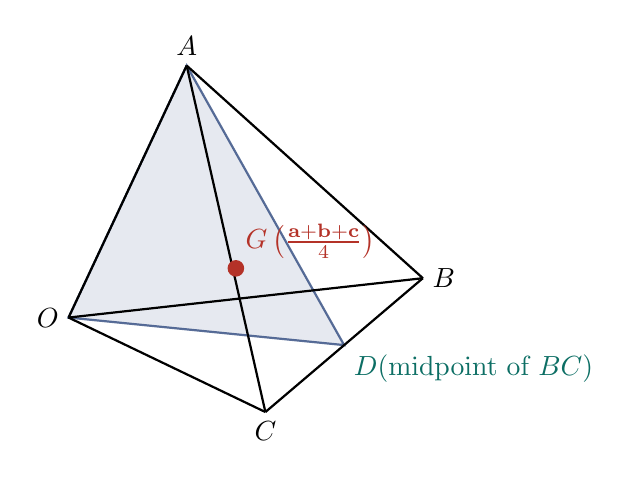
\begin{tikzpicture}[scale=1.0, >=Stealth]
  % Tetrahedron vertices
  \coordinate (O) at (0, 0);
  \coordinate (A) at (1.5, 3.2);
  \coordinate (B) at (4.5, 0.5);
  \coordinate (C) at (2.5, -1.2);
  
  % Midpoint of BC
  \coordinate (D) at ($(B)!0.5!(C)$);
  
  % Centroid G
  \coordinate (G) at (2.125, 0.625);
  
  % Shaded median plane OAD
  \draw[fill=primary!15, opacity=0.7, draw=primary, thick] (O) -- (A) -- (D) -- cycle;
  
  % Edges of tetrahedron
  \draw[thick] (O) -- (A);
  \draw[thick] (O) -- (B);
  \draw[thick] (O) -- (C);
  \draw[thick] (A) -- (B);
  \draw[thick] (B) -- (C);
  \draw[thick] (A) -- (C);
  
  % Labels
  \node[left] at (O) {$O$};
  \node[above] at (A) {$A$};
  \node[right] at (B) {$B$};
  \node[below] at (C) {$C$};
  \node[below right, secondary] at (D) {$D (\text{midpoint of } BC)$};
  
  % Centroid G
  \fill[accent] (2.125, 0.625) circle (3pt) node[above right, font=\bfseries\color{accent}]{$G \left(\frac{\mathbf{a}+\mathbf{b}+\mathbf{c}}{4}\right)$};
\end{tikzpicture}
\end{center}

\vspace{0.4cm}
\hrule
\vspace{0.4cm}

% =========================================================================
% PROBLEM 19
% =========================================================================
\section{Problem 19}
\begin{problembox}[Problem 19]
A variable plane which remains at a constant distance $p$ from the origin, cuts the coordinate axes in $A, B, C$. Show that:
\begin{enumerate}
    \item[(i)] the locus of the centroid of the triangle $ABC$ is $\dfrac{1}{x^2} + \dfrac{1}{y^2} + \dfrac{1}{z^2} = \dfrac{9}{p^2}$
    \item[(ii)] the locus of the centroid of the tetrahedron $OABC$ is $\dfrac{1}{x^2} + \dfrac{1}{y^2} + \dfrac{1}{z^2} = \dfrac{16}{p^2}$
\end{enumerate}
\end{problembox}

\paragraph{Proof:}
Let the intercepts of the variable plane on the coordinate axes be $A(a, 0, 0), B(0, b, 0), C(0, 0, c)$. The equation of the plane is:
$$\frac{x}{a} + \frac{y}{b} + \frac{z}{c} = 1$$
The perpendicular distance from the origin $(0, 0, 0)$ to this plane is given by $p$:
$$p = \frac{|0 - 1|}{\sqrt{\frac{1}{a^2} + \frac{1}{b^2} + \frac{1}{c^2}}} = \frac{1}{\sqrt{\frac{1}{a^2} + \frac{1}{b^2} + \frac{1}{c^2}}}$$
Squaring both sides and inverting:
$$\frac{1}{a^2} + \frac{1}{b^2} + \frac{1}{c^2} = \frac{1}{p^2} \qquad \text{--- (Equation 1)}$$

\paragraph{Part (i): Locus of the centroid of $\triangle ABC$.}
Let $(\xi, \eta, \zeta)$ be the coordinates of the centroid of $\triangle ABC$:
$$\xi = \frac{a + 0 + 0}{3} = \frac{a}{3} \implies a = 3\xi$$
$$\eta = \frac{0 + b + 0}{3} = \frac{b}{3} \implies b = 3\eta$$
$$\zeta = \frac{0 + 0 + c}{3} = \frac{c}{3} \implies c = 3\zeta$$
Substituting $a, b, c$ into Equation (1):
$$\frac{1}{(3\xi)^2} + \frac{1}{(3\eta)^2} + \frac{1}{(3\zeta)^2} = \frac{1}{p^2} \implies \frac{1}{9}\left(\frac{1}{\xi^2} + \frac{1}{\eta^2} + \frac{1}{\zeta^2}\right) = \frac{1}{p^2}$$
$$\frac{1}{\xi^2} + \frac{1}{\eta^2} + \frac{1}{\zeta^2} = \frac{9}{p^2}$$
Generalizing to current coordinates $(x, y, z)$, the locus is:
$$\frac{1}{x^2} + \frac{1}{y^2} + \frac{1}{z^2} = \frac{9}{p^2} \qquad \text{\checkmark (Proved)}$$

\paragraph{Part (ii): Locus of the centroid of tetrahedron $OABC$.}
Let $(\xi, \eta, \zeta)$ be the centroid of the tetrahedron $OABC$ ($O$ being $(0,0,0)$):
$$\xi = \frac{0 + a + 0 + 0}{4} = \frac{a}{4} \implies a = 4\xi$$
$$\eta = \frac{0 + 0 + b + 0}{4} = \frac{b}{4} \implies b = 4\eta$$
$$\zeta = \frac{0 + 0 + 0 + c}{4} = \frac{c}{4} \implies c = 4\zeta$$
Substituting into Equation (1):
$$\frac{1}{(4\xi)^2} + \frac{1}{(4\eta)^2} + \frac{1}{(4\zeta)^2} = \frac{1}{p^2} \implies \frac{1}{16}\left(\frac{1}{\xi^2} + \frac{1}{\eta^2} + \frac{1}{\zeta^2}\right) = \frac{1}{p^2}$$
$$\frac{1}{\xi^2} + \frac{1}{\eta^2} + \frac{1}{\zeta^2} = \frac{16}{p^2}$$
Generalizing to $(x, y, z)$, the locus is:
$$\frac{1}{x^2} + \frac{1}{y^2} + \frac{1}{z^2} = \frac{16}{p^2} \qquad \text{\checkmark (Proved)}$$

\vspace{0.4cm}
\hrule
\vspace{0.4cm}

% =========================================================================
% PROBLEM 20
% =========================================================================
\section{Problem 20}
\begin{problembox}[Problem 20]
A variable plane passes through a fixed point $a\hat{i} + b\hat{j} + c\hat{k}$ and meets the coordinate axes in $A, B, C$. Show that the locus of the point common to the planes through $A, B, C$ parallel to the coordinate planes is
$$\frac{a}{x} + \frac{b}{y} + \frac{c}{z} = 1$$
\end{problembox}

\paragraph{Proof:}
Let the equation of the variable plane in intercept form be:
$$\frac{x}{\alpha} + \frac{y}{\beta} + \frac{z}{\gamma} = 1$$
where $\alpha, \beta, \gamma$ are the variable intercepts on the axes. Thus:
$$A = (\alpha, 0, 0), \quad B = (0, \beta, 0), \quad C = (0, 0, \gamma)$$

Since this plane passes through the fixed point $(a, b, c)$, its coordinates must satisfy the plane equation:
$$\frac{a}{\alpha} + \frac{b}{\beta} + \frac{c}{\gamma} = 1 \qquad \text{--- (Equation 1)}$$

Now consider the planes through $A, B, C$ drawn parallel to the coordinate planes:
\begin{itemize}
    \item Through $A(\alpha, 0, 0)$ parallel to the $yz$-plane ($x=0$): Equation is $x = \alpha$.
    \item Through $B(0, \beta, 0)$ parallel to the $zx$-plane ($y=0$): Equation is $y = \beta$.
    \item Through $C(0, 0, \gamma)$ parallel to the $xy$-plane ($z=0$): Equation is $z = \gamma$.
\end{itemize}
The common point of intersection of these three planes is $P(x, y, z) = (\alpha, \beta, \gamma)$.\\
Therefore:
$$\alpha = x, \quad \beta = y, \quad \gamma = z$$
Substituting these into Equation (1), we obtain the locus:
$$\frac{a}{x} + \frac{b}{y} + \frac{c}{z} = 1$$
This completes the proof. \qed

\vspace{0.4cm}
\hrule
\vspace{0.4cm}

% =========================================================================
% PROBLEM 21
% =========================================================================
\section{Problem 21}
\begin{problembox}[Problem 21]
Through a point $P(a, b, c)$, a plane is drawn at right angles to $OP$ to meet the coordinate axes in $A, B, C$; $O$ being the origin. Prove that the area of the triangle $ABC$ is $\dfrac{p^5}{2abc}$, where $OP = p$.
\end{problembox}

\paragraph{Proof:}
\textbf{Step 1: Equation of the plane through $P$ perpendicular to $OP$.}\\
Given $P(a, b, c)$, the distance $OP = p$ satisfies:
$$p^2 = a^2 + b^2 + c^2$$
The normal vector is $\vec{OP} = a\hat{i} + b\hat{j} + c\hat{k}$. The plane passing through $P(a, b, c)$ is:
$$a(x - a) + b(y - b) + c(z - c) = 0 \implies ax + by + cz = a^2 + b^2 + c^2 = p^2$$

\textbf{Step 2: Intercepts on the coordinate axes.}\\
Writing the plane in intercept form:
$$\frac{x}{p^2/a} + \frac{y}{p^2/b} + \frac{z}{p^2/c} = 1$$
Thus, the vertices of $\triangle ABC$ are:
$$A\left(\frac{p^2}{a}, 0, 0\right), \quad B\left(0, \frac{p^2}{b}, 0\right), \quad C\left(0, 0, \frac{p^2}{c}\right)$$

\textbf{Step 3: Area of $\triangle ABC$ via projections.}\\
Let $\Delta$ be the area of $\triangle ABC$, and let $\Delta_x, \Delta_y, \Delta_z$ be the areas of the projections of $\triangle ABC$ on the $yz$, $zx$, and $xy$ coordinate planes respectively.
By the projection theorem for areas in 3D:
$$\Delta^2 = \Delta_x^2 + \Delta_y^2 + \Delta_z^2$$
Each projection is a right-angled triangle at the origin:
\begin{itemize}
    \item Projection on $yz$-plane is $\triangle OBC$: $\Delta_x = \frac{1}{2}\left(\frac{p^2}{b}\right)\left(\frac{p^2}{c}\right) = \frac{p^4}{2bc}$
    \item Projection on $zx$-plane is $\triangle OCA$: $\Delta_y = \frac{1}{2}\left(\frac{p^2}{a}\right)\left(\frac{p^2}{c}\right) = \frac{p^4}{2ac}$
    \item Projection on $xy$-plane is $\triangle OAB$: $\Delta_z = \frac{1}{2}\left(\frac{p^2}{a}\right)\left(\frac{p^2}{b}\right) = \frac{p^4}{2ab}$
\end{itemize}
Now sum their squares:
$$\Delta^2 = \left(\frac{p^4}{2bc}\right)^2 + \left(\frac{p^4}{2ac}\right)^2 + \left(\frac{p^4}{2ab}\right)^2 = \frac{p^8}{4a^2b^2c^2}\left(a^2 + b^2 + c^2\right)$$
Since $a^2 + b^2 + c^2 = p^2$:
$$\Delta^2 = \frac{p^8}{4a^2b^2c^2} \cdot p^2 = \frac{p^{10}}{4a^2b^2c^2}$$
Taking the square root:
$$\Delta = \frac{p^5}{2abc}$$
Hence, the area of $\triangle ABC$ is $\dfrac{p^5}{2abc}$. \qed
\begin{center}
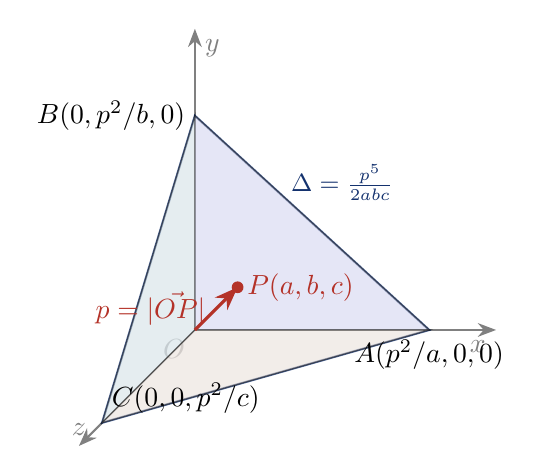
\begin{tikzpicture}[scale=0.85, >=Stealth]
  % Axes
  \draw[->, thick, gray] (0,0,0) -- (4.5,0,0) node[anchor=north east]{$x$};
  \draw[->, thick, gray] (0,0,0) -- (0,4.5,0) node[anchor=north west]{$y$};
  \draw[->, thick, gray] (0,0,0) -- (0,0,4.5) node[anchor=south]{$z$};
  \node[below left] at (0,0,0) {$O$};
  
  % Points A, B, C
  \coordinate (A) at (3.5, 0, 0);
  \coordinate (B) at (0, 3.2, 0);
  \coordinate (C) at (0, 0, 3.6);
  
  % Plane ABC
  \draw[fill=primary!15, opacity=0.75, draw=primary, thick] (A) -- (B) -- (C) -- cycle;
  
  % Projections
  \draw[fill=blue!10, opacity=0.5] (0,0,0) -- (A) -- (B) -- cycle;
  \draw[fill=teal!10, opacity=0.5] (0,0,0) -- (B) -- (C) -- cycle;
  \draw[fill=orange!10, opacity=0.5] (0,0,0) -- (A) -- (C) -- cycle;
  
  % Normal OP
  \coordinate (P) at (1.1, 1.1, 1.2);
  \draw[->, very thick, accent] (0,0,0) -- (P) node[midway, left]{$p = |\vec{OP}|$};
  \fill[accent] (P) circle (2.5pt) node[right]{$P(a,b,c)$};
  
  \node[below] at (A) {$A(p^2/a, 0, 0)$};
  \node[left] at (B) {$B(0, p^2/b, 0)$};
  \node[above right] at (C) {$C(0, 0, p^2/c)$};
  \node[font=\bfseries\small, primary] at (2.2, 2.2, 0) {$\Delta = \frac{p^5}{2abc}$};
\end{tikzpicture}
\end{center}


\vspace{0.4cm}
\hrule
\vspace{0.4cm}

% =========================================================================
% PROBLEM 22
% =========================================================================
\section{Problem 22}
\begin{problembox}[Problem 22]
Perpendiculars $PL, PM, PN$ are drawn from the point $P(a, b, c)$ to the coordinate planes; find the equation of the plane $LMN$.
\end{problembox}

\paragraph{Step 1: Find the feet of perpendiculars $L, M, N$.}
\begin{itemize}
    \item $PL \perp yz$-plane ($x = 0$): Foot is $L(0, b, c)$.
    \item $PM \perp zx$-plane ($y = 0$): Foot is $M(a, 0, c)$.
    \item $PN \perp xy$-plane ($z = 0$): Foot is $N(a, b, 0)$.
\end{itemize}

\paragraph{Step 2: Determine the equation of plane $LMN$.}
Let the plane equation be $Ax + By + Cz + D = 0$. Since $L, M, N$ lie on the plane:
\begin{align}
    B b + C c + D &= 0 \implies B b + C c = -D \label{eq:lmn1}\\
    A a + C c + D &= 0 \implies A a + C c = -D \label{eq:lmn2}\\
    A a + B b + D &= 0 \implies A a + B b = -D \label{eq:lmn3}
\end{align}
Subtracting \eqref{eq:lmn1} from \eqref{eq:lmn2}: $A a - B b = 0 \implies A a = B b$.\\
Subtracting \eqref{eq:lmn2} from \eqref{eq:lmn3}: $B b - C c = 0 \implies B b = C c$.\\
Thus, $A a = B b = C c = k$ (a constant).\\
From \eqref{eq:lmn3}: $k + k = -D \implies D = -2k$.\\
Therefore:
$$A = \frac{k}{a}, \quad B = \frac{k}{b}, \quad C = \frac{k}{c}, \quad D = -2k$$
Substituting into $Ax + By + Cz + D = 0$:
$$\frac{k}{a}x + \frac{k}{b}y + \frac{k}{c}z - 2k = 0$$
Dividing by $k \neq 0$:
$$\frac{x}{a} + \frac{y}{b} + \frac{z}{c} = 2 \iff \frac{x}{a} + \frac{y}{b} + \frac{z}{c} - 2 = 0$$

\begin{resultbox}
\textbf{Final Answer:}\\
$\boxed{\frac{x}{a} + \frac{y}{b} + \frac{z}{c} = 2}$ \quad (or $bc x + ca y + ab z = 2abc$)
\end{resultbox}

\vspace{0.4cm}
\hrule
\vspace{0.4cm}

% =========================================================================
% PROBLEM 23
% =========================================================================
\section{Problem 23}
\begin{problembox}[Problem 23]
The plane $lx + my = 0$ is rotated about its line of intersection with the plane $z = 0$, through an angle $\alpha$. Prove that its equation in its new position is
$$lx + my \pm z\sqrt{l^2 + m^2}\tan\alpha = 0$$
\end{problembox}

\paragraph{Proof:}
The line of intersection of the plane $lx + my = 0$ and the plane $z = 0$ is the line $lx + my = 0, z = 0$.
Any plane passing through this line of intersection belongs to the family:
$$lx + my + \lambda z = 0 \qquad \text{--- (1)}$$

The normal vector to the initial plane $lx + my = 0$ is:
$$\mathbf{n}_0 = l\hat{i} + m\hat{j} + 0\hat{k}, \qquad |\mathbf{n}_0| = \sqrt{l^2 + m^2}$$
The normal vector to the new plane (1) is:
$$\mathbf{n} = l\hat{i} + m\hat{j} + \lambda\hat{k}, \qquad |\mathbf{n}| = \sqrt{l^2 + m^2 + \lambda^2}$$

Since the plane has rotated through an angle $\alpha$, the angle between $\mathbf{n}$ and $\mathbf{n}_0$ is $\alpha$:
$$\cos\alpha = \frac{\mathbf{n} \cdot \mathbf{n}_0}{|\mathbf{n}||\mathbf{n}_0|} = \frac{l^2 + m^2}{\sqrt{l^2 + m^2 + \lambda^2}\sqrt{l^2 + m^2}} = \frac{\sqrt{l^2 + m^2}}{\sqrt{l^2 + m^2 + \lambda^2}}$$
Squaring both sides:
$$\cos^2\alpha = \frac{l^2 + m^2}{l^2 + m^2 + \lambda^2} \implies \sec^2\alpha = \frac{l^2 + m^2 + \lambda^2}{l^2 + m^2} = 1 + \frac{\lambda^2}{l^2 + m^2}$$
Using the trigonometric identity $\sec^2\alpha - 1 = \tan^2\alpha$:
$$\tan^2\alpha = \frac{\lambda^2}{l^2 + m^2} \implies \lambda^2 = (l^2 + m^2)\tan^2\alpha$$
$$\lambda = \pm \sqrt{l^2 + m^2}\tan\alpha$$
Substituting $\lambda$ back into (1):
$$lx + my \pm z\sqrt{l^2 + m^2}\tan\alpha = 0$$
This completes the proof. \qed
\begin{center}
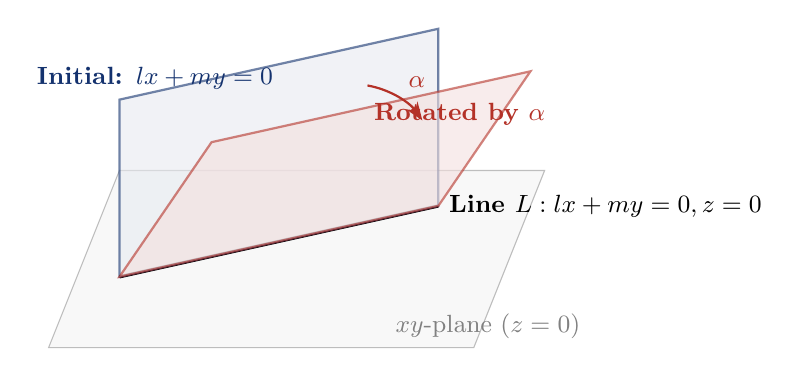
\begin{tikzpicture}[scale=0.9, >=Stealth]
  % xy plane
  \draw[fill=gray!10, opacity=0.5, draw=gray] (-3, -1.5) -- (3, -1.5) -- (4, 1) -- (-2, 1) -- cycle;
  \node[gray, font=\small] at (3.2, -1.2) {$xy$-plane ($z=0$)};
  
  % Line of intersection L
  \draw[very thick, black] (-2, -0.5) -- (2.5, 0.5) node[right, font=\bfseries\small]{Line $L: lx+my=0, z=0$};
  
  % Original vertical plane P0
  \draw[fill=primary!10, opacity=0.6, draw=primary, thick] (-2, -0.5) -- (2.5, 0.5) -- (2.5, 3) -- (-2, 2) -- cycle;
  \node[primary, font=\small\bfseries] at (-1.5, 2.3) {Initial: $lx+my=0$};
  
  % Rotated plane P
  \draw[fill=accent!15, opacity=0.6, draw=accent, thick] (-2, -0.5) -- (2.5, 0.5) -- (3.8, 2.4) -- (-0.7, 1.4) -- cycle;
  \node[accent, font=\small\bfseries] at (2.8, 1.8) {Rotated by $\alpha$};
  
  % Rotation arc
  \draw[->, thick, accent] (1.5, 2.2) arc (80:35:1.2) node[midway, above right, font=\small\bfseries]{$\alpha$};
\end{tikzpicture}
\end{center}


\vspace{0.4cm}
\hrule
\vspace{0.4cm}

% =========================================================================
% PROBLEM 24
% =========================================================================
\section{Problem 24}
\begin{problembox}[Problem 24]
Show that the combined equation of the two planes inclined at an angle $\alpha$ to the $xy$-plane and containing the line $y = 0, \, z\cos\beta = x\sin\beta$ is
$$z^2 + (x^2 + y^2)\tan^2\beta - 2zx\tan\beta = y^2\tan^2\alpha$$
\end{problembox}

\paragraph{Proof:}
The given line of intersection is:
$$y = 0, \quad z\cos\beta - x\sin\beta = 0 \iff x\tan\beta - z = 0$$
Any plane containing this line is represented by:
$$(x\tan\beta - z) + \lambda y = 0 \iff x\tan\beta + \lambda y - z = 0 \qquad \text{--- (1)}$$

The normal vector to this plane is:
$$\mathbf{n} = (\tan\beta)\hat{i} + \lambda\hat{j} - \hat{k}$$
The normal to the $xy$-plane ($z = 0$) is $\mathbf{n}_0 = \hat{k}$.\\
Since the plane is inclined at an angle $\alpha$ to the $xy$-plane:
$$\cos\alpha = \frac{|\mathbf{n} \cdot \hat{k}|}{|\mathbf{n}||\hat{k}|} = \frac{|-1|}{\sqrt{\tan^2\beta + \lambda^2 + (-1)^2} \cdot 1} = \frac{1}{\sqrt{1 + \tan^2\beta + \lambda^2}}$$
Squaring and inverting:
$$\sec^2\alpha = 1 + \tan^2\beta + \lambda^2$$
Since $\sec^2\alpha = 1 + \tan^2\alpha$:
$$1 + \tan^2\alpha = 1 + \tan^2\beta + \lambda^2 \implies \lambda^2 = \tan^2\alpha - \tan^2\beta$$

From the plane equation (1), express $\lambda$:
$$\lambda y = z - x\tan\beta \implies \lambda = \frac{z - x\tan\beta}{y}$$
Squaring this expression:
$$\lambda^2 = \frac{(z - x\tan\beta)^2}{y^2}$$
Equating both expressions for $\lambda^2$:
$$\frac{(z - x\tan\beta)^2}{y^2} = \tan^2\alpha - \tan^2\beta$$
Multiplying by $y^2$:
$$(z - x\tan\beta)^2 = y^2(\tan^2\alpha - \tan^2\beta)$$
Expanding the left side:
$$z^2 - 2zx\tan\beta + x^2\tan^2\beta = y^2\tan^2\alpha - y^2\tan^2\beta$$
Adding $y^2\tan^2\beta$ to the left side:
$$z^2 + (x^2 + y^2)\tan^2\beta - 2zx\tan\beta = y^2\tan^2\alpha$$
This is the combined equation of the two planes. \qed

\vspace{0.4cm}
\hrule
\vspace{0.4cm}

% =========================================================================
% PROBLEM 25
% =========================================================================
\section{Problem 25}
\begin{problembox}[Problem 25]
Use vector method to show that the plane whose intercepts on the three coordinate axes are $a, b$ and $c$ respectively, divides the line segment joining the origin to the point $a\hat{i} + b\hat{j} + c\hat{k}$ internally in the ratio $1 : 2$.
\end{problembox}

\paragraph{Proof:}
Let $O(\mathbf{0})$ be the origin and $P(\mathbf{p})$ be the given point, where $\mathbf{p} = a\hat{i} + b\hat{j} + c\hat{k}$.\\
The equation of the plane whose intercepts on the coordinate axes are $a, b, c$ is:
$$\frac{x}{a} + \frac{y}{b} + \frac{z}{c} = 1$$
In vector form, letting $\mathbf{n} = \dfrac{1}{a}\hat{i} + \dfrac{1}{b}\hat{j} + \dfrac{1}{c}\hat{k}$:
$$\mathbf{r} \cdot \mathbf{n} = 1$$

Let a point $R$ divide the line segment $OP$ internally in the ratio $k : 1$. By the section formula:
$$\mathbf{r}_R = \frac{k\mathbf{p} + 1\cdot\mathbf{0}}{k + 1} = \frac{k}{k + 1}(a\hat{i} + b\hat{j} + c\hat{k})$$

Since $R$ lies on the plane, $\mathbf{r}_R$ must satisfy the plane equation $\mathbf{r}_R \cdot \mathbf{n} = 1$:
$$\left[\frac{k}{k + 1}(a\hat{i} + b\hat{j} + c\hat{k})\right] \cdot \left(\frac{1}{a}\hat{i} + \frac{1}{b}\hat{j} + \frac{1}{c}\hat{k}\right) = 1$$
Evaluating the scalar product:
$$\frac{k}{k + 1}\left(a \cdot \frac{1}{a} + b \cdot \frac{1}{b} + c \cdot \frac{1}{c}\right) = 1$$
$$\frac{k}{k + 1}(1 + 1 + 1) = 1 \implies \frac{3k}{k + 1} = 1$$
$$3k = k + 1 \implies 2k = 1 \implies k = \frac{1}{2}$$
Therefore, the ratio is:
$$\frac{k}{1} = \frac{1/2}{1} = \frac{1}{2} \iff 1 : 2$$
Thus, the plane divides the line segment joining the origin to $a\hat{i} + b\hat{j} + c\hat{k}$ internally in the ratio $1 : 2$. \qed
\begin{center}
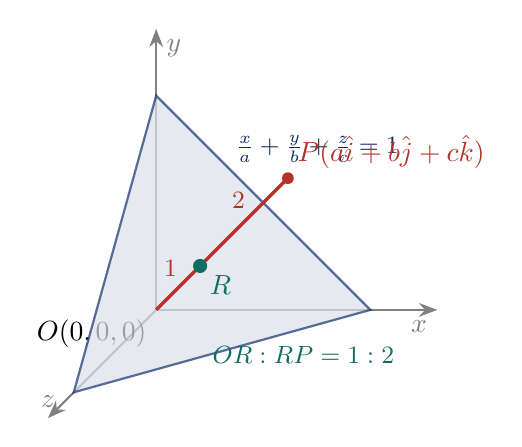
\begin{tikzpicture}[scale=0.85, >=Stealth]
  % Axes
  \draw[->, thick, gray] (0,0,0) -- (4.2,0,0) node[anchor=north east]{$x$};
  \draw[->, thick, gray] (0,0,0) -- (0,4.2,0) node[anchor=north west]{$y$};
  \draw[->, thick, gray] (0,0,0) -- (0,0,4.2) node[anchor=south]{$z$};
  \node[below left] at (0,0,0) {$O(0,0,0)$};
  
  % Intercepts
  \coordinate (A) at (3.2, 0, 0);
  \coordinate (B) at (0, 3.2, 0);
  \coordinate (C) at (0, 0, 3.2);
  
  % Shaded Plane
  \draw[fill=primary!15, opacity=0.7, draw=primary, thick] (A) -- (B) -- (C) -- cycle;
  \node[primary!90!black, font=\small\bfseries] at (2.6, 2.6, 0.5) {$\frac{x}{a}+\frac{y}{b}+\frac{z}{c}=1$};
  
  % Point P(a, b, c) and line segment OP
  \coordinate (P) at (3.2, 3.2, 3.2);
  \draw[very thick, accent] (0,0,0) -- (P);
  \fill[accent] (P) circle (2.5pt) node[above right]{$P(a\hat{i}+b\hat{j}+c\hat{k})$};
  
  % Intersection Point R on the plane
  \coordinate (R) at (1.067, 1.067, 1.067);
  \fill[secondary] (R) circle (3pt) node[below right, font=\bfseries\color{secondary}]{$R$};
  
  % Ratio annotations
  \node[accent, font=\bfseries\small] at (0.35, 0.75, 0.35) {$1$};
  \node[accent, font=\bfseries\small] at (2.0, 2.4, 2.0) {$2$};
  \node[below, font=\small\color{secondary}] at (2.2, -0.4, 0) {$OR : RP = 1 : 2$};
\end{tikzpicture}
\end{center}


\vspace{0.4cm}
\hrule
\vspace{0.4cm}

% =========================================================================
% PROBLEM 26
% =========================================================================
\section{Problem 26}
\begin{problembox}[Problem 26]
Find the equation of the plane passing through the intersection of the planes $2x + 5y - 5z = 6$ and $2x + 7y - 8z = 7$ and the point $(-1, 4, 3)$.
\end{problembox}

\paragraph{Step 1: Family of planes through the line of intersection.}
The family of planes passing through the intersection of the two planes is:
$$(2x + 5y - 5z - 6) + \lambda(2x + 7y - 8z - 7) = 0$$

\paragraph{Step 2: Determine $\lambda$ using the point $(-1, 4, 3)$.}
Substitute $x = -1, y = 4, z = 3$:
$$[2(-1) + 5(4) - 5(3) - 6] + \lambda[2(-1) + 7(4) - 8(3) - 7] = 0$$
$$[-2 + 20 - 15 - 6] + \lambda[-2 + 28 - 24 - 7] = 0$$
$$-3 + \lambda(-5) = 0 \implies -3 - 5\lambda = 0 \implies \lambda = -\frac{3}{5}$$

\paragraph{Step 3: Substitute $\lambda$ and simplify.}
$$(2x + 5y - 5z - 6) - \frac{3}{5}(2x + 7y - 8z - 7) = 0$$
Multiplying by $5$:
$$5(2x + 5y - 5z - 6) - 3(2x + 7y - 8z - 7) = 0$$
$$(10x + 25y - 25z - 30) - (6x + 21y - 24z - 21) = 0$$
$$(10 - 6)x + (25 - 21)y + (-25 + 24)z + (-30 + 21) = 0$$
$$4x + 4y - z - 9 = 0 \iff 4x + 4y - z = 9$$

\begin{resultbox}
\textbf{Final Answer:}\\
$\boxed{4x + 4y - z - 9 = 0}$ \quad or \quad $\boxed{4x + 4y - z = 9}$
\end{resultbox}

\vspace{0.4cm}
\hrule
\vspace{0.4cm}

% =========================================================================
% PROBLEM 27
% =========================================================================
\section{Problem 27}
\begin{problembox}[Problem 27]
Find the locus of a point the sum of squares of whose distances from the planes $x + y + z = 0, \, x - 2y + z = 0$ is equal to the square of its distance from the plane $x - z = 0$.
\end{problembox}

\paragraph{Step 1: Compute perpendicular distances.}
Let $P(x, y, z)$ be the variable point.
\begin{itemize}
    \item Distance $d_1$ from $x + y + z = 0$:
    $$d_1 = \frac{|x + y + z|}{\sqrt{1^2 + 1^2 + 1^2}} = \frac{|x + y + z|}{\sqrt{3}} \implies d_1^2 = \frac{(x + y + z)^2}{3}$$
    \item Distance $d_2$ from $x - 2y + z = 0$:
    $$d_2 = \frac{|x - 2y + z|}{\sqrt{1^2 + (-2)^2 + 1^2}} = \frac{|x - 2y + z|}{\sqrt{6}} \implies d_2^2 = \frac{(x - 2y + z)^2}{6}$$
    \item Distance $d_3$ from $x - z = 0$:
    $$d_3 = \frac{|x - z|}{\sqrt{1^2 + 0^2 + (-1)^2}} = \frac{|x - z|}{\sqrt{2}} \implies d_3^2 = \frac{(x - z)^2}{2}$$
\end{itemize}

\paragraph{Step 2: Equate $d_1^2 + d_2^2 = d_3^2$.}
$$\frac{(x + y + z)^2}{3} + \frac{(x - 2y + z)^2}{6} = \frac{(x - z)^2}{2}$$
Multiply the entire equation by $6$:
$$2(x + y + z)^2 + (x - 2y + z)^2 = 3(x - z)^2$$

\paragraph{Step 3: Algebraic expansion and simplification.}
Let $u = x + z$. Then $x + y + z = u + y$ and $x - 2y + z = u - 2y$:
$$2(u + y)^2 + (u - 2y)^2 = 2(u^2 + 2uy + y^2) + (u^2 - 4uy + 4y^2)$$
$$= 2u^2 + 4uy + 2y^2 + u^2 - 4uy + 4y^2 = 3u^2 + 6y^2$$
Now, rewrite $u^2 = (x + z)^2 = x^2 + 2xz + z^2$:
$$3u^2 + 6y^2 = 3(x^2 + 2xz + z^2) + 6y^2 = 3x^2 + 6xz + 3z^2 + 6y^2$$
The right-hand side is:
$$3(x - z)^2 = 3(x^2 - 2xz + z^2) = 3x^2 - 6xz + 3z^2$$
Equating both sides:
$$3x^2 + 6xz + 3z^2 + 6y^2 = 3x^2 - 6xz + 3z^2$$
Subtracting $3x^2 + 3z^2$ from both sides:
$$6xz + 6y^2 = -6xz \implies 6y^2 + 12xz = 0 \implies y^2 + 2xz = 0$$

\begin{resultbox}
\textbf{Final Answer:}\\
$\boxed{y^2 + 2xz = 0}$
\end{resultbox}

\vspace{0.4cm}
\hrule
\vspace{0.4cm}

% =========================================================================
% PROBLEM 28
% =========================================================================
\section{Problem 28}
\begin{problembox}[Problem 28]
Find the equations of the planes through the points $(0, 4, -3), \, (6, -4, 3)$ other than the plane through the origin, which cut off from the axes intercepts whose sum is zero.
\end{problembox}

\paragraph{Step 1: Intercept form and given condition.}
Let the non-zero intercepts made by the plane on the coordinate axes be $a, b, c$.
$$\frac{x}{a} + \frac{y}{b} + \frac{z}{c} = 1$$
Given that the sum of the intercepts is zero:
$$a + b + c = 0 \implies c = -(a + b)$$
Thus the equation becomes:
$$\frac{x}{a} + \frac{y}{b} - \frac{z}{a + b} = 1 \qquad \text{--- (1)}$$

\paragraph{Step 2: Substitute the two given points.}
\begin{enumerate}
    \item Point $(0, 4, -3)$:
    $$\frac{0}{a} + \frac{4}{b} - \frac{-3}{a + b} = 1 \implies \frac{4}{b} + \frac{3}{a + b} = 1 \qquad \text{--- (2)}$$
    \item Point $(6, -4, 3)$:
    $$\frac{6}{a} - \frac{4}{b} - \frac{3}{a + b} = 1 \implies \frac{6}{a} - \left(\frac{4}{b} + \frac{3}{a + b}\right) = 1 \qquad \text{--- (3)}$$
\end{enumerate}
From equation (2), substitute $\left(\dfrac{4}{b} + \dfrac{3}{a + b}\right) = 1$ into equation (3):
$$\frac{6}{a} - 1 = 1 \implies \frac{6}{a} = 2 \implies a = 3$$

\paragraph{Step 3: Solve for $b$ and $c$.}
Substitute $a = 3$ into equation (2):
$$\frac{4}{b} + \frac{3}{3 + b} = 1 \implies \frac{4(3 + b) + 3b}{b(3 + b)} = 1$$
$$12 + 4b + 3b = 3b + b^2 \implies b^2 - 4b - 12 = 0$$
Factoring:
$$(b - 6)(b + 2) = 0 \implies b = 6 \quad \text{or} \quad b = -2$$

\paragraph{Step 4: Find the equations for both cases.}
\begin{itemize}
    \item \textbf{Case 1: $a = 3, b = 6$}\\
    $c = -(a + b) = -(3 + 6) = -9$.\\
    Equation: $\dfrac{x}{3} + \dfrac{y}{6} - \dfrac{z}{9} = 1$.\\
    Multiplying by $18$:
    $$6x + 3y - 2z = 18 \iff 6x + 3y - 2z - 18 = 0$$
    
    \item \textbf{Case 2: $a = 3, b = -2$}\\
    $c = -(a + b) = -(3 - 2) = -1$.\\
    Equation: $\dfrac{x}{3} - \dfrac{y}{2} - \dfrac{z}{1} = 1$.\\
    Multiplying by $6$:
    $$2x - 3y - 6z = 6 \iff 2x - 3y - 6z - 6 = 0$$
\end{itemize}

\begin{resultbox}
\textbf{Final Answer:}\\
There are two such planes:\\
$\boxed{6x + 3y - 2z = 18}$ \quad and \quad $\boxed{2x - 3y - 6z = 6}$
\end{resultbox}

\vspace{0.4cm}
\hrule
\vspace{0.4cm}

% =========================================================================
% PROBLEM 29
% =========================================================================
\section{Problem 29}
\begin{problembox}[Problem 29]
Find the equation of the plane through the line of intersection of the planes $ax + by + cz + d = 0, \, a_1 x + b_1 y + c_1 z + d_1 = 0$ and parallel to the $x$-axis.
\end{problembox}

\paragraph{Step 1: Family of planes through the intersection.}
The family of planes passing through the intersection of the two planes is:
$$(ax + by + cz + d) + \lambda(a_1 x + b_1 y + c_1 z + d_1) = 0$$
$$(a + \lambda a_1)x + (b + \lambda b_1)y + (c + \lambda c_1)z + (d + \lambda d_1) = 0$$
The normal vector of this plane is:
$$\mathbf{n} = (a + \lambda a_1)\hat{i} + (b + \lambda b_1)\hat{j} + (c + \lambda c_1)\hat{k}$$

\paragraph{Step 2: Condition for parallelism to the $x$-axis.}
The $x$-axis has direction vector $\hat{i} = (1, 0, 0)$.\\
Since the plane is parallel to the $x$-axis, its normal vector $\mathbf{n}$ must be perpendicular to $\hat{i}$:
$$\mathbf{n} \cdot \hat{i} = 0 \implies a + \lambda a_1 = 0 \implies \lambda = -\frac{a}{a_1} \quad (a_1 \neq 0)$$

\paragraph{Step 3: Substitute $\lambda$ and simplify.}
$$(ax + by + cz + d) - \frac{a}{a_1}(a_1 x + b_1 y + c_1 z + d_1) = 0$$
Multiplying by $a_1$:
$$a_1(ax + by + cz + d) - a(a_1 x + b_1 y + c_1 z + d_1) = 0$$
$$(a a_1 - a a_1)x + (a_1 b - a b_1)y + (a_1 c - a c_1)z + (a_1 d - a d_1) = 0$$
$$(a_1 b - a b_1)y + (a_1 c - a c_1)z + (a_1 d - a d_1) = 0$$
Equivalently:
$$(a b_1 - a_1 b)y + (a c_1 - a_1 c)z + (a d_1 - a_1 d) = 0$$

\begin{resultbox}
\textbf{Final Answer:}\\
$\boxed{(a_1 b - a b_1)y + (a_1 c - a c_1)z + (a_1 d - a d_1) = 0}$\\
or equivalently: $\boxed{(a b_1 - a_1 b)y + (a c_1 - a_1 c)z + (a d_1 - a_1 d) = 0}$
\end{resultbox}

\vspace{0.4cm}
\hrule
\vspace{0.4cm}

% =========================================================================
% PROBLEM 30
% =========================================================================
\section{Problem 30}
\begin{problembox}[Problem 30]
A triangle, the lengths of whose sides are $a, b, c$ is placed so that the middle points of the sides are on the axes. Prove that the equation to its plane is
$$\frac{x}{\alpha} + \frac{y}{\beta} + \frac{z}{\gamma} = 1$$
\end{problembox}

\paragraph{Proof:}
\textbf{Step 1: Coplanarity of the triangle and its midpoints.}\\
Let the triangle be $\triangle PQR$ having side lengths:
$$QR = a, \quad RP = b, \quad PQ = c$$
Let $D, E, F$ be the midpoints of the sides $QR, RP, PQ$ respectively.
Since the vertices $P, Q, R$ lie in a plane $\Pi$, the midpoints $D, E, F$ of its sides must also lie in the same plane $\Pi$.

\textbf{Step 2: Coordinates of the midpoints on the axes.}\\
The problem specifies that the midpoints of the sides lie on the coordinate axes:
\begin{itemize}
    \item Midpoint $D$ lies on the $x$-axis $\implies D(\alpha, 0, 0)$
    \item Midpoint $E$ lies on the $y$-axis $\implies E(0, \beta, 0)$
    \item Midpoint $F$ lies on the $z$-axis $\implies F(0, 0, \gamma)$
\end{itemize}
Since the three non-collinear points $D(\alpha, 0, 0)$, $E(0, \beta, 0)$, $F(0, 0, \gamma)$ lie on the coordinate axes and also lie in the plane $\Pi$, the plane $\Pi$ has intercepts $\alpha, \beta, \gamma$ on the $x, y, z$ axes respectively.

The equation of a plane in intercept form with intercepts $\alpha, \beta, \gamma$ is:
$$\frac{x}{\alpha} + \frac{y}{\beta} + \frac{z}{\gamma} = 1$$

\textbf{Step 3: Relationship between intercepts $\alpha, \beta, \gamma$ and side lengths $a, b, c$.}\\
By the Midpoint Theorem in plane geometry, the segment joining the midpoints of any two sides of a triangle is parallel to the third side and has length equal to half of that side:
$$EF = \frac{1}{2}QR = \frac{a}{2}, \qquad FD = \frac{1}{2}RP = \frac{b}{2}, \qquad DE = \frac{1}{2}PQ = \frac{c}{2}$$
Using the 3D distance formula between points $D(\alpha, 0, 0), E(0, \beta, 0), F(0, 0, \gamma)$:
\begin{align}
    EF^2 &= (0 - 0)^2 + (\beta - 0)^2 + (0 - \gamma)^2 = \beta^2 + \gamma^2 = \frac{a^2}{4} \label{eq:m1}\\
    FD^2 &= (\alpha - 0)^2 + (0 - 0)^2 + (0 - \gamma)^2 = \alpha^2 + \gamma^2 = \frac{b^2}{4} \label{eq:m2}\\
    DE^2 &= (\alpha - 0)^2 + (0 - \beta)^2 + (0 - 0)^2 = \alpha^2 + \beta^2 = \frac{c^2}{4} \label{eq:m3}
\end{align}
Summing equations \eqref{eq:m1}, \eqref{eq:m2}, and \eqref{eq:m3}:
$$2(\alpha^2 + \beta^2 + \gamma^2) = \frac{a^2 + b^2 + c^2}{4} \implies \alpha^2 + \beta^2 + \gamma^2 = \frac{a^2 + b^2 + c^2}{8}$$
Subtracting equation \eqref{eq:m1} ($\beta^2 + \gamma^2 = \frac{a^2}{4}$):
$$\alpha^2 = \frac{a^2 + b^2 + c^2}{8} - \frac{a^2}{4} = \frac{b^2 + c^2 - a^2}{8} \iff 8\alpha^2 = b^2 + c^2 - a^2$$
Similarly:
$$8\beta^2 = c^2 + a^2 - b^2, \qquad 8\gamma^2 = a^2 + b^2 - c^2$$
This explicitly determines the intercepts $\alpha, \beta, \gamma$ in terms of the side lengths $a, b, c$. Hence, the equation to the plane of the triangle is:
$$\frac{x}{\alpha} + \frac{y}{\beta} + \frac{z}{\gamma} = 1$$
This completes the proof. \qed

\begin{center}
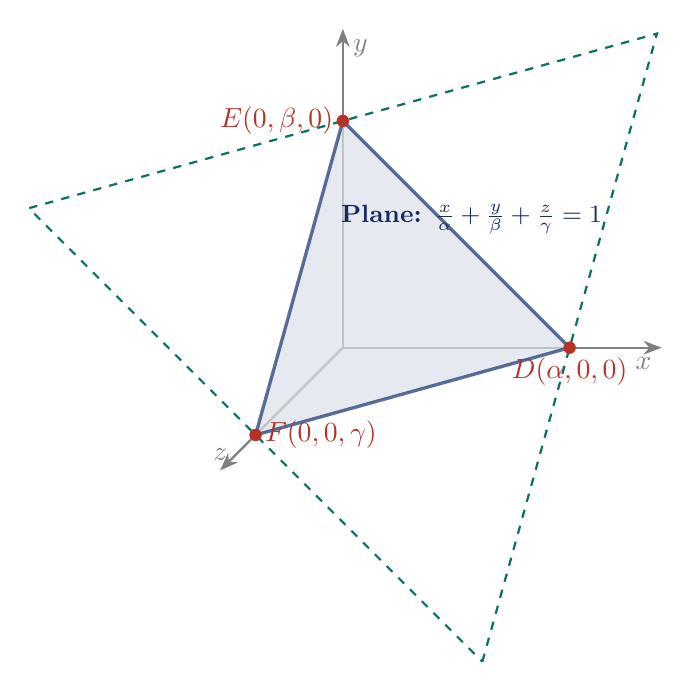
\begin{tikzpicture}[scale=0.9, >=Stealth]
  % Axes
  \draw[->, thick, gray] (0,0,0) -- (4.5,0,0) node[anchor=north east]{$x$};
  \draw[->, thick, gray] (0,0,0) -- (0,4.5,0) node[anchor=north west]{$y$};
  \draw[->, thick, gray] (0,0,0) -- (0,0,4.5) node[anchor=south]{$z$};
  
  % Midpoints on axes
  \coordinate (D) at (3.2, 0, 0);
  \coordinate (E) at (0, 3.2, 0);
  \coordinate (F) at (0, 0, 3.2);
  
  % Shaded Plane DEF
  \draw[fill=primary!15, opacity=0.7, draw=primary, very thick] (D) -- (E) -- (F) -- cycle;
  
  % Vertices of Triangle PQR (extended)
  \coordinate (P) at (3.2, -3.2, 3.2);
  \coordinate (Q) at (3.2, 3.2, -3.2);
  \coordinate (R) at (-3.2, 3.2, 3.2);
  
  \draw[dashed, thick, secondary] (P) -- (Q) -- (R) -- cycle;
  
  % Marks
  \fill[accent] (D) circle (2.5pt) node[below]{$D(\alpha, 0, 0)$};
  \fill[accent] (E) circle (2.5pt) node[left]{$E(0, \beta, 0)$};
  \fill[accent] (F) circle (2.5pt) node[right]{$F(0, 0, \gamma)$};
  
  \node[primary!90!black, font=\bfseries\small] at (2.2, 2.2, 1) {Plane: $\frac{x}{\alpha}+\frac{y}{\beta}+\frac{z}{\gamma}=1$};
\end{tikzpicture}
\end{center}

\vspace{0.4cm}
\begin{resultbox}
\textbf{Conclusion:}\\
The midpoints of the sides lie in the plane of the triangle with intercepts $\alpha, \beta, \gamma$ on the coordinate axes. Therefore, the equation to its plane is:
$$\boxed{\frac{x}{\alpha} + \frac{y}{\beta} + \frac{z}{\gamma} = 1}$$
where $8\alpha^2 = b^2 + c^2 - a^2, \quad 8\beta^2 = c^2 + a^2 - b^2, \quad 8\gamma^2 = a^2 + b^2 - c^2$.
\end{resultbox}

\end{document}
